% multiple1902 <multiple1902@gmail.com>
% master.tex
% Copyright 2011~2012, multiple1902 (Weisi Dai)
% https://code.google.com/p/xjtuthesis/
%
% It is strongly recommended that you read documentations located at
%   http://code.google.com/p/xjtuthesis/wiki/Landing?tm=6
% in advance of your compilation if you have not read them before.
%
% This work may be distributed and/or modified under the
% conditions of the LaTeX Project Public License, either version 1.3
% of this license or (at your option) any later version.
% The latest version of this license is in
%   http://www.latex-project.org/lppl.txt
% and version 1.3 or later is part of all distributions of LaTeX
% version 2005/12/01 or later.
%
% This work has the LPPL maintenance status `maintained'.
%
% The Current Maintainer of this work is Weisi Dai.
%
\documentclass[
    master,
    truefont, % just turn it on when using Windows
    %nofont, % remember to manally set the fonts
    pdflinks,
    %colorlinks,
    % compact,
    ]{xjtuthesis}

\usepackage{threeparttable}
\usepackage{tabularx}
\usepackage{tikz}
\usepackage{listings}
\usepackage{algorithm}
\usepackage{algorithmic}


\definecolor{dkgreen}{rgb}{0,0.6,0}
\definecolor{gray}{rgb}{0.5,0.5,0.5}
\definecolor{mauve}{rgb}{0.58,0,0.82}

\lstset{ %
  language=Octave,                % the language of the code
  basicstyle=\small,           % the size of the fonts that are used for the code
  %numbers=left,                   % where to put the line-numbers
  numberstyle=\tiny\color{gray},  % the style that is used for the line-numbers
  stepnumber=2,                   % the step between two line-numbers. If it's 1, each line
                                  % will be numbered
  numbersep=5pt,                  % how far the line-numbers are from the code
  backgroundcolor=\color{white},      % choose the background color. You must add \usepackage{color}
  showspaces=false,               % show spaces adding particular underscores
  showstringspaces=false,         % underline spaces within strings
  showtabs=false,                 % show tabs within strings adding particular underscores
  frame=single,                   % adds a frame around the code
  rulecolor=\color{black},        % if not set, the frame-color may be changed on line-breaks within not-black text (e.g. commens (green here))
  tabsize=2,                      % sets default tabsize to 2 spaces
  captionpos=b,                   % sets the caption-position to bottom
  breaklines=true,                % sets automatic line breaking
  breakatwhitespace=false,        % sets if automatic breaks should only happen at whitespace
  title=\lstname,                   % show the filename of files included with \lstinputlisting;
                                  % also try caption instead of title
  keywordstyle=\color{blue},          % keyword style
  commentstyle=\color{dkgreen},       % comment style
  stringstyle=\color{mauve},         % string literal style
  escapeinside={\%*}{*)},            % if you want to add LaTeX within your code
  morekeywords={*,...}               % if you want to add more keywords to the set
}

\usetikzlibrary{shapes.geometric, arrows}

\hyphenation{op-tical net-works semi-conduc-tor}

\graphicspath{{figures/}}

\begin{document}

    % 请修改 meta.tex 中的论文元信息
    % multiple1902 <multiple1902@gmail.com>
% meta.tex
% Copyright 2011~2012, multiple1902 (Weisi Dai)
% https://code.google.com/p/xjtuthesis/
%
% It is strongly recommended that you read documentations located at
%   http://code.google.com/p/xjtuthesis/wiki/Landing?tm=6
% in advance of your compilation if you have not read them before.
%
% This work may be distributed and/or modified under the
% conditions of the LaTeX Project Public License, either version 1.3
% of this license or (at your option) any later version.
% The latest version of this license is in
%   http://www.latex-project.org/lppl.txt
% and version 1.3 or later is part of all distributions of LaTeX
% version 2005/12/01 or later.
%
% This work has the LPPL maintenance status `maintained'.
%
% The Current Maintainer of this work is Weisi Dai.
%

% 标题,中文
\ctitle{基于由粗到细的场景文字检测方法研究与应用}

% 作者,中文
\cauthor{贺翔 }

% 学科,中文,本科生不需要
\csubject{软件工程}

% 导师姓名,中文
\csupervisor{宋永红 \quad 高级工程师}

% 关键词,中文。用全角分号「;」分割
% 研究生的应首先从《汉语主题词表》中摘选
\ckeywords{场景文字检测;由粗到细;文字边缘骨架切割;统计边缘响应;二叉树搜索}

% 提交日期,本科生不需要
\cproddate{\the\year 年\the\month 月}

% 论文类型,中文,本科生不需要
% 从理论研究、应用基础、应用研究、研究报告、软件开发、设计报告、案例分析、调研报告、其它中选择
\ctype{应用研究}

% 论文标题,英文
\etitle{Research and Application of Coarse-to-fine Scene text detection}

% 作者姓名,英文
\eauthor{Xiang He }

% 学科,英文,本科生不需要
\esubject{Software Engineering}

% 导师姓名,英文
\esupervisor{Senior Engineer Yonghong Song }

% 关键词,英文。用半角分号和一个半角空格「; 」分割
\ekeywords{scene text detection; coarse to fine; text Skeleton-cut; Static skeleton response; Binary tree based Search}

% 学科门类,英文
% 从Philosophy(哲学)、Economics(经济学)、Law (法学)、Education(教育学)、Arts(文学)、
%   Science(理学)、Engineering Science(工学)、Medicine(医学)、Management Science(管理学)中选择
\ecate{Engineering Science}

% 提交日期,英文,本科生不需要
% 应当和 cproddate 保持一致
\eproddate{\monthname{\month}\ \the\year}

% 论文类型,英文,本科生不需要
% 从Theoretical Research(理论研究)、Application Fundamentals (应用基础)、Applied Research(应用研究)、
%   Research Report(研究报告)、Software Development(软件开发)、Design Report(设计报告)、
%   Case Study(案例分析)、Investigation Report (调研报告)、其它(Other)中选择
\etype{Applied Research}

% 摘要,中文。段间空行
\cabstract{

}

% 摘要,英文。段间空行
\eabstract{

}

    \xjtuchead
    \xjtuehead
    \xjtucinfopage
    \xjtueinfopage
    \xjtutoc
    \xjtutoe
    \clearpage

    % 主要符号表,可以没有
    %% multiple1902 <multiple1902@gmail.com>
% denotation.tex
% Copyright 2011~2012, multiple1902 (Weisi Dai)
% https://code.google.com/p/xjtuthesis/
%
% It is strongly recommended that you read documentations located at
%   http://code.google.com/p/xjtuthesis/wiki/Landing?tm=6
% in advance of your compilation if you have not read them before.
%
% This work may be distributed and/or modified under the
% conditions of the LaTeX Project Public License, either version 1.3
% of this license or (at your option) any later version.
% The latest version of this license is in
%   http://www.latex-project.org/lppl.txt
% and version 1.3 or later is part of all distributions of LaTeX
% version 2005/12/01 or later.
%
% This work has the LPPL maintenance status `maintained'.
%
% The Current Maintainer of this work is Weisi Dai.
%
\begin{denotation}
    \iffalse
        \item[符号1]    解释1
        \item[符号2]    解释2
    \fi
\end{denotation}


    \xjtucontent
        % multiple1902 <multiple1902@gmail.com>
% intro.tex
% Copyright 2011~2012, multiple1902 (Weisi Dai)
% https://code.google.com/p/xjtuthesis/
%
% It is strongly recommended that you read documentations located at
%   http://code.google.com/p/xjtuthesis/wiki/Landing?tm=6
% in advance of your compilation if you have not read them before.
%
% This work may be distributed and/or modified under the
% conditions of the LaTeX Project Public License, either version 1.3
% of this license or (at your option) any later version.
% The latest version of this license is in
%   http://www.latex-project.org/lppl.txt
% and version 1.3 or later is part of all distributions of LaTeX
% version 2005/12/01 or later.
%
% This work has the LPPL maintenance status `maintained'.
%
% The Current Maintainer of this work is Weisi Dai.
%

\chapter{绪论}
\echapter{Introduction}

本章主要对本文研究内容的背景和意义进行介绍,以及对国内外研究在此领域的现状进行讨论,并给出本文的主要研究内容和组织结构。

    \section{背景}
    \esection{Background}

    文字是用来存储信息或记录语言的图像符号,图像中的文字是可以直接传递内容语义的重要信息源,而让计算机能够定位并理解数字图像中的文字,即文字检测和识别,直到现在仍是图像处理与模式识别领域中的研究热点。其对于图像检索,盲人辅助系统,无人驾驶导航及文档图像处理等人工智能系统均起到巨大的辅助作用,如图\ref{fig.c1_apply}所示:

    \begin{figure*}[!h]
    \centering
    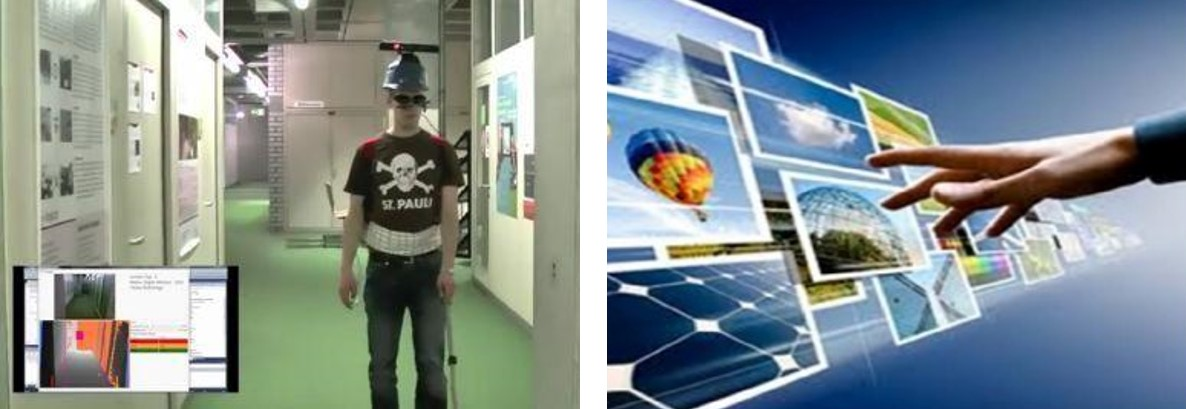
\includegraphics[width=\textwidth]{./figures/c1_apply_1.jpg}
    \begin{minipage}[t]{0.48\linewidth}
    \centerline{ \small (a) 盲人辅助设备}
    \end{minipage}
    \begin{minipage}[t]{0.48\linewidth}
    \centerline{ \small (b) 基于内容的海量图像检索}
    \end{minipage}
    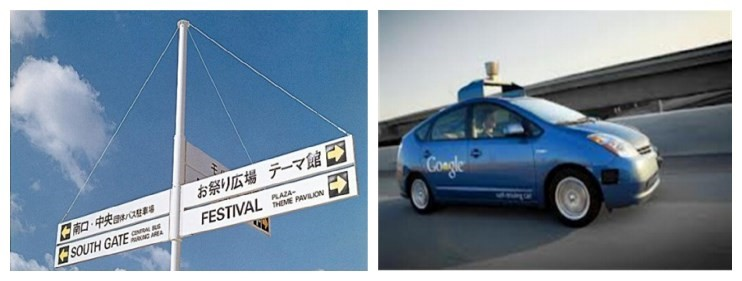
\includegraphics[width=\textwidth]{./figures/c1_apply_2.jpg}
    \begin{minipage}[t]{0.48\linewidth}
    \centerline{ \small (d) 国外旅游辅助}
    \end{minipage}
    \begin{minipage}[t]{0.48\linewidth}
    \centerline{ \small (e) 无人驾驶导航系统}
    \end{minipage}
    \caption{自然场景中文字检测与识别的应用}
    \label{fig.c1_apply}
    \end{figure*}

    在图像信息检索方面,通过计算机自动获取图像中可能存在的文字信息,可帮助计算机理解图像内容,实现对图像的自动标注,从而辅助图像搜索引擎,视频网站等工程场景的建设;在文档图像处理系统方面,可应用于淘宝、大众点评等门户网站,通过对顾客或商家上传的大量图像文件如发票、许可证书等进行文字检测和识别,可对图像进行自动判别和归类,以取代耗时耗力的人工审核;无人驾驶导航系统需要从无人驾驶汽车所处的道路环境中收集有效信息,并规划出从起点到终点的最优路径,而检测及提取出道路上标识牌中的文字信息,往往是无人驾驶导航系统能够安全、合法地行驶的必要条件;盲人辅助系统同样可通过文字检测获取标识牌及周围环境的文字信息,并通过文字识别将文字信息转换为语音或其它行驶的信息来辅助盲人获取环境信息。

    文字检测根据文字的存储媒介的不同又可分为不同类型如视频文字检测,自然场景图像文字检测等。其中,自然场景图像是指由人工拍摄而非计算机直接生成的图像。自然场景中拍摄的图像,其图像质量易受拍摄环境及拍摄条件的影响,背景较为复杂,图像中文字的字体、颜色及形态多变,这些因素都使得自然场景图像中的文字检测较为困难,呈现如图 \ref{fig.c1_problem} 所示的一些需要解决的难题:

    \begin{figure*}[!h]
    \centering
    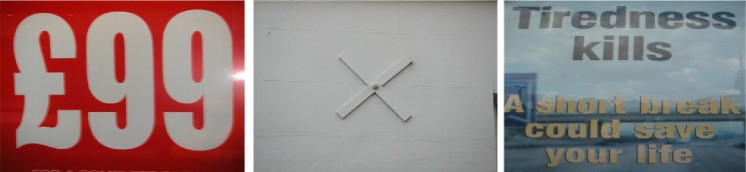
\includegraphics[width=\textwidth]{./figures/c1_problem_1.jpg}
    \begin{minipage}[t]{0.31\linewidth}
    \centerline{ \small (a) 多尺度}
    \end{minipage}
    \begin{minipage}[t]{0.31\linewidth}
    \centerline{ \small (b) 对比度低}
    \end{minipage}
    \begin{minipage}[t]{0.31\linewidth}
    \centerline{ \small (c) 不同颜色}
    \end{minipage}
    
\includegraphics[width=\textwidth]{./figures/c1_problem_2.jpg}
    \begin{minipage}[t]{0.31\linewidth}
    \centerline{ \small (d) 不均匀光照}
    \end{minipage}
    \begin{minipage}[t]{0.31\linewidth}
    \centerline{ \small (e) 排列方向多变}
    \end{minipage}
    \begin{minipage}[t]{0.31\linewidth}
    \centerline{ \small (f) 复杂背景}
    \end{minipage}
    \caption{自然场景文字领域的挑战}
    \label{fig.c1_problem}
    \end{figure*}

    这些挑战包括:复杂的自然场景:在自然环境中,有许多类似文字的人为目标,例如建筑、标志和绘画等。复杂的自然场景使得文字难以从背景中被区分开来;对比度过低:文字通常与背景有一定的对比度以便于人类识别。但是某些时候,文字可能与背景有非常相似的纹理和颜色,这时文字就难以被分辨出来;不均匀的光照:由于图像采集时的光照影响和图像采集设备的不均匀响应,会使图像中产生不均匀的光照,有时图像过暗,有时图像局部太亮。不均匀光照会引入颜色失真和恶化的视觉特征,从而导致错误的分割和检测结果;排列方向多变 自然场景图像中的文字不仅是水平或竖直排列,也会倾斜排列或者曲线排列。不同的排列方向使得文字检测需要考虑更多情况从而变得困难;多语种:世界上的语种数量较多,常见的有英文、中文、日文、阿拉伯文等。不同语种的文字有不同的特点,使得在进行文字检测识别时需要考虑很多不同情况。在自然场景中进行多语种文字检测识别是非常困难的;图像模糊和退化:由于图像采集时多变的工作条件和自动对焦的使用,散焦和模糊的自然图像时常会产生。图像压缩和解压也会影响图像的质量,特别是图像中的文字。图像散焦、模糊和退化会降低文字的锐度使得文字粘连在一起,使得文字分割检测变得更加困难;图像失真:当图像采集时图像采集设备如相机等的光轴不垂直于文字所在平面时会产生透视变形。文字包围盒不是矩形和字符扭曲,都会使失真的文字难以被检测出来。

    近年来在文字检测与识别领域,研究者们为解决上述难题做了大量的研究和探索,提出了大量的文字检测方法,检测结果也在逐年提高。但目前的方法在ICDAR公开测试集上的测评结果表明,自然场景图像中的文字检测和识别效果仍有提升空间。

    \section{国内外研究现状}
    \esection{Related Work}
    
    自然场景图像中的文字检测和识别是计算机视觉领域的研究热点,国内外的很多学者在从事该方面的研究,他们也提出了很多的方法来解决这个问题,而Ye 等人\cite{Ye2015Text}对这些方法进行了调研和总结。 同时,在国际会议ICDAR 上举办了多次关于文字检测的比赛“Robust Reading”\cite{Karatzas2013ICDAR},自然场景中的文字检测及识别就是其中的一项比赛内容,不仅为从事文字检测方面研究的人提供了交流的机会,而且也反映了当时文字检测的最先进水平。
    
    自然场景图像中的文字检测方法按照其处理对象的不同,可分为基于纹理的方法和基于区域的方法:基于纹理的文字检测方法,把文字当作一种特殊纹理,通常通过局部颜色对比度、笔划滤波器、频域变换等方法来刻画文字的纹理特征。在确定纹理特征提取方式之后,往往会使用各种分类模型训练文字-背景分类器,以滑动窗的形式判断图像局部区域内是否包含文字,由此生成文字概率图。之后通过聚类或图像分割等方法取得候选文字行或文字区域,再经过后处理生成最终的检测结果。为检测不同尺寸的文字,基于纹理的方法往往需要在输入图像的不同尺度的图像上都进行同样的纹理特征提取和区域分类,或设计不同大小的纹理特征提取模板在同一个滑动窗内提取多次特征,并进行多尺度的结果融合。因此这类方法比较耗时;基于区域的文字检测方法,通常利用文字具有与背景差异明显且均一的颜色这一特征,从输入图像中提取出有限个数的候选文字区域,然后使用一些经验性的规则,或者提取区域的几何、纹理等特征,使用分类模型来滤除掉背景区域。基于区域的方法通常要比基于纹理的方法效率更高,因为基于区域的方法需要处理的区域数目有限。但这类方法的缺点在于,文字区域由于光照、遮挡、模糊等原因,内部颜色分布差异变大,或者边缘模糊,往往会在提取候选文字区域时被漏检,会直接影响最终检测结果。
    
    2010年,Epshtein\cite{Epshtein2010Detecting}等人提出了笔画宽度变换(SWT)来计算图像中每个像素的笔画,基于像素笔画产生候选文字连通区域,去掉非文字连通区域就得到文字检测结果。笔画是组成文字的基本元素,通过计算笔画来检测文字是文字检测中非常有意义的研究进展;2011年,Neumann和Matas\cite{Neumann2011Text} 使用最稳定极值区域(MSER)作为候选文字区域,通过有效剪枝可以详尽搜索所有可能文字序列,并利用高阶文字属性(文字行)对候选区域进行区分从而确定文字区域;2012 年,Tu\cite{Tu2012Detecting}等提出了一种检测自然图像中任意方向的文字的方法,他们使用SWT来获得候选文字连通区域,然后通过单个连通区域的分析和连通区域行的分析来去掉非文字部分,保留下来的连通区域就是文字检测的结果;2014年,Yin\cite{Yin2013Robust}等设计了一个快速有效的剪枝算法来提取图像中的最稳定机制区域(MSER)作为候选文字连通区域,他们通过一个单链聚类算法将候选文字链接成候选文字行,这个聚类算法的距离权重和聚类阈值是通过一个自训练距离度量学习算法自动学习到的,通过贝叶斯模型利用字符分类器计算候选文字的后验概率,从而将文字检测出来;2015年,Yu\cite{Yu2015Text} 等提出了一种基于边缘分析的文字检测方法,他们使用边缘重组来产生候选文字连通区域,然后通过单个连通区域分析、连通区域行分析对候选文字进行验证,得到最终的文字检测结果。
    
    近些年,随着深度学习\cite{Moral2010Foundations}的兴起,它被广泛用于目标检测识别任务,例如手写字符识别、交通标志识别等,同时取得了非常好的结果,大大提升了目标检测识别的水平。鉴于深度学习的良好表现,许多人也将深度学习用于自然场景中的文字检测。

    \section{本文研究内容}
    \esection{Research Contents}

    \section{论文的组织结构}
    \esection{Thesis Structure}



        %% multiple1902 <multiple1902@gmail.com>
% intro.tex
% Copyright 2011~2012, multiple1902 (Weisi Dai)
% https://code.google.com/p/xjtuthesis/
%
% It is strongly recommended that you read documentations located at
%   http://code.google.com/p/xjtuthesis/wiki/Landing?tm=6
% in advance of your compilation if you have not read them before.
%
% This work may be distributed and/or modified under the
% conditions of the LaTeX Project Public License, either version 1.3
% of this license or (at your option) any later version.
% The latest version of this license is in
%   http://www.latex-project.org/lppl.txt
% and version 1.3 or later is part of all distributions of LaTeX
% version 2005/12/01 or later.
%
% This work has the LPPL maintenance status `maintained'.
%
% The Current Maintainer of this work is Weisi Dai.
%

\chapter{论文相关理论与技术}
\echapter{Relative Theory and Technology}

    文字检测按照其研究目标和存储介质的不同,可分为数字图像文字检测、视频图像中的文字检测和自然场景图像中的文字检测。其中,由于自然场景中的文字会遭受背景复杂多样性,以及图像质量易被光照、阴影、遮挡等环境因素影响,致使自然场景图像的文字检测相比于其它图像对检测算法的健壮性要求更高。这些年来,学者们在文字检测领域进行了大量的研究和实验工作,提出了许多不同的方法,检测效果也在逐年提升。但是在ICDAR等公开数据集上的测试结果表明,目前的这些自然场景图像中的文字检测结果仍有提高空间,所以仍是文字检测领域内的一个热点方向。场景图像文字检测方法根据流程不同,可分为基于区域的文字检测方法和基于连通部件的文字检测方法两大类。下面整理并分别介绍近年来这两类文字检测的相关方法。

    \section{基于区域的场景文字检测方法}
    \esection{Region-based Method}

    基于区域的文字检测方法,是基于文子有别于背景的视觉特征来区分文字区域与背景区域的。使用较多的视觉特征主要包括纹理、边缘及颜色等。因为每个文字都是用来传递信息的特定符号,其纹理与一般背景并不相同,同时文字相比于背景也有着更强的对比度和显著的颜色,所以包含着文字的那些区域和背景图像区域有着不同的视觉特征,因而可以用来区分文字区域与非文字区域。

    大部分基于区域的方法一般都会利用滑动窗来获取候选的包含文字的局部图像区域,因此在有些方法中也称其为基于滑动窗的文字检测算法。如图\ref{fig.c2_region_based} 所示,这是1个典型的基于区域的文字检测方法的流程示例。在该流程示例中,首先利用滑动窗来得到局部图像区域以作为候选区域,然后提取区域中的颜色、纹理等视觉特征,最后结合分类器以进行文字与非文字区域的分类判别,输出结果是检测出来的文字区域。

    \begin{figure}[!h]
    \centering
    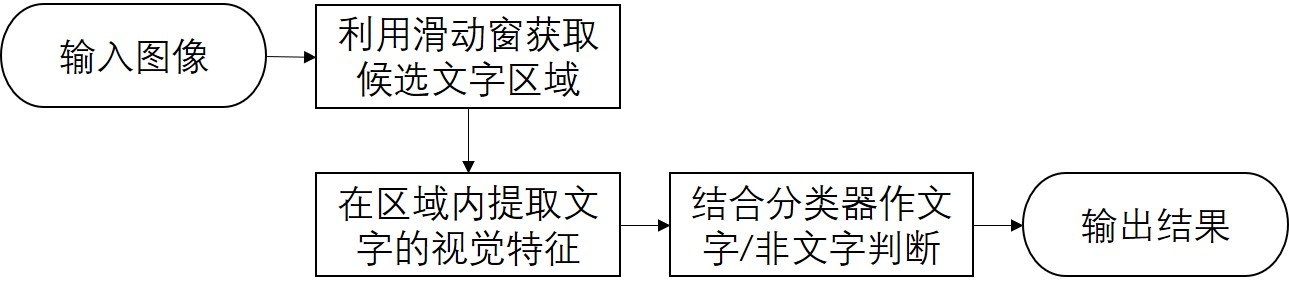
\includegraphics[width=\textwidth]{c2_region_based.jpg}
    \caption{基于区域的文字检测方法的流程示例}
    \label{fig.c2_region_based}
    \end{figure}

    Chen等\cite{Chen2004Detecting}利用滑动窗扫描得到文字区域并获取区域中的79个特征,然后构造4个级联的Adaboost 分类器来分类和筛选这些候选文字区域,最后用OCR软件识别图像中文字信息。其中4个级联的分类器是由不同的文字底层特征构造而成的弱分类器,通过利用Adaboost方法将这些弱分类器组合学习而获得1 个分类文字与背景的强分类器。用于训练弱分类器的三组特征分别是:候选区域内竖直和水平方向灰度的标准差与平均值;区域内的统计梯度信息;区域内边缘组合特征。而本方法中使用的79个特征,分散在4层的级联分类器中,分别有1、10、30和50维文字特征。最后OCR使用的技术是用Niblack方法来二值化检测到的文字区域以识别出图像中的文字。

    Pan等\cite{Pan2011A}设计了一种基于滑动窗的文本区域的检测器,用于估算图像金字塔中的文本行存在的置信度和尺度信息,在每个尺度中使用滑动窗扩得到候选文字区域并利用WaldBoost分了器对各个窗口的文字置信度进行预测。然后该文利用基于连通部件类别中的局部二值化方法对候选文本分量进行分割。为有效的过滤掉非文本的部件,这篇文章提出了一个考虑一元组件的属性和二元上下文的成分关系的条件随机场(CRF)模型。其中,一元特征表征单个部件自身的文字置信度,例如有占空比、紧密度、轮廓梯度以及宽高比等;而二元特征表征相邻候选文字连通部件即上下文的关系,如颜色、形状、尺度和距离等差异。最后基于能量最小化方法将这些文本组件分类到文本行中。

    上述文字检测方法一般使用人工设计的特征,例如颜色、纹理、笔画宽度等,进行文字与非文字分类。虽然这些特征可以区分大多数的文字与非文字,部分与文字相似的背景却难以区分,例如窗户、砖块等。为了能够更好地反映文字的属性,近年来许多方法开始采用深度学习技术,其中最常用的一种结构是卷积神经网络(CNN)。CNN是一种特殊的前馈人工神经网络,其中的神经元之间的连接关系类似于视觉皮层的结构。同时,因为CNN能够利用图像中的局部空间相关性,故CNN特别适合于处理计算机视觉问题,尤其是目标识别领域,例如在手写字符识别、交通标志识别、图像分类等方面都取得了优秀的表现。

    \begin{figure}[!h]
    \centering
    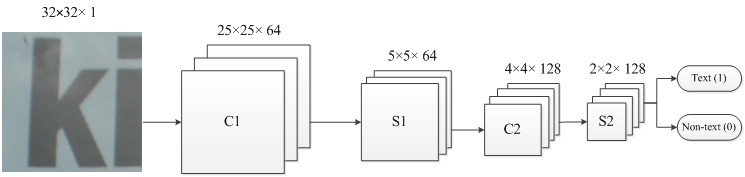
\includegraphics[width=\textwidth]{c2_wangtao_cnn.jpg}
    \caption{Wang等\cite{Wang2012End}采用的CNN网络框架}
    \label{fig.c2_wangtao_cnn}
    \end{figure}

    Wang等\cite{Wang2012End}设计的端对端文字检测和识别框架的核心即是卷积神经网络CNN。该方法首先利用滑动窗在图像金字塔上扫描得到候选文字图像块区域,然后将这些图像块区域缩放成$32\times32$像素大小的正方形小图块。接着这些图块的灰度图会输入到1个训练好的,含有2层卷积的CNN网络中进行特征的提取,以及对这些图块区域的分类。其中,卷积神经网络CNN的结构如图\ref{fig.c2_wangtao_cnn}所示:输入图像小块经过第1层的64个卷积模板的卷积操作后,得到64个$25\times25$的响应图,紧接着再执行平均池化获得相应的$5\times5$ 的响应;然后再通过第2卷积层中的128个卷积模板的卷积操作及后续的平均池化操作后,得到$2\times2\times128$的全连接层。在通过上CNN 网络的特征提取和分类后,最后再利用非极大抑制NMS操作来筛选重叠的分类结果以获得文字行定位结果。此外还构建62类的分类器来识别图块中的文字。

    \begin{figure*}[!h]
    \centering
    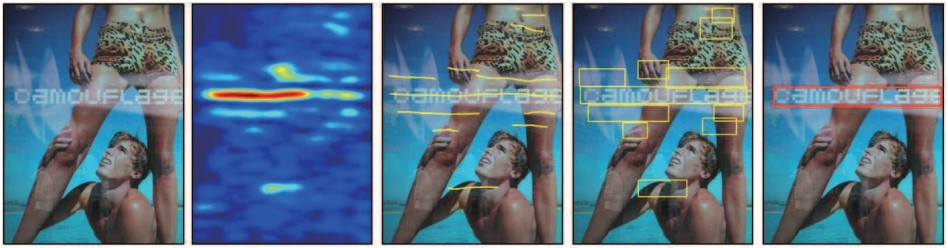
\includegraphics[width=\textwidth]{./figures/c2_zhang_cnn.jpg}
    \begin{minipage}[t]{0.18\linewidth}
    \centerline{ \small (a) 输入原图}
    \end{minipage}
    \begin{minipage}[t]{0.18\linewidth}
    \centerline{ \small (b) 概率图}
    \end{minipage}
    \begin{minipage}[t]{0.18\linewidth}
    \centerline{ \small (c) 对称轴}
    \end{minipage}
    \begin{minipage}[t]{0.18\linewidth}
    \centerline{ \small (d) 候选文本行}
    \end{minipage}
    \begin{minipage}[t]{0.18\linewidth}
    \centerline{ \small (d) CNN分类结果}
    \end{minipage}
    \caption{基于对称性文本行检测算法流程}
    \label{fig.c2_zhang_cnn}
    \end{figure*}

    Zhang等\cite{Zhang2015Symmetry}提出一种利用滑动窗提取对称性特征的文字检测算法。该方法首先设计1个对称性计算模板来计算滑动窗口内区域的梯度直方图、局部二值模式LBP以及颜色等特征的相似度,然后将这些特征输入随机森林分类器从而得到每个像素属于文本行对称轴的概率图。接着把概率图上概率相近的像素集中形成文本行对称轴并用CRF进行更准确的分类。然后在此基础上利用窗口尺寸生成候选文本行并作多个尺度上的文本行的投影融合。最后采用训练好的CNN分类器去掉非文字的图像区域。从这个方法的实验结果来看,利用深度学习来分类候选文本行区域,可将其中真实的文字部分精准的辨别出来,因而能较大程度的提高文本检测的成绩。

    \begin{table*}[!h]
    \centering
    \caption{基于区域的相关文字检测方法}
    \begin{tabular}{p{0.17\textwidth}|p{0.1\textwidth}| p{0.63\textwidth}}
    \hline
    作者 & 年份 & 方法概述 \\
    \hline
    Chen等\cite{Chen2004Detecting} & 2004年 & 区域特征,滑动窗检测,以及SVM分类器;\\
    Pan等\cite{Pan2011A} & 2011年 &   条件随机场,滑动窗检测,以及waldBoost分类器\\
    Wang等\cite{Wang2012End} & 2012年 & 卷积神经网络和滑动窗检测 \\
    Zhang等\cite{Zhang2015Symmetry} & 2015年 & 对称性特征,滑动窗检测以及卷积神经网络 \\
    \hline
    \end{tabular}
    \label{tab.c2_region_based}
    \end{table*}

    表格\ref{tab.c2_region_based}总结了基于区域的相关文字检测方法。(优缺点;wang的方法的问题:第3章的问题提出;zhang的方法中怎么利用CNN,对我的方法的启发)

    \section{基于连通部件的场景文字检测方法}
    \esection{Connected Component-based Method}

    基于连通部件的检测方法,将文字看做是一些连通部件的集合,所以这类方法是把连通部件作为处理对象的文字检测算法。这种基于连通部件来检测场景图像中文字的原理是:因为文字之间的笔画、纹理、对比度以及颜色等特征具有一致性,所以可通过笔画宽度转换、图像分割或最稳定极值区域提取等处理,来把候选文字的像素组成一系列的连通部件。

    \begin{figure}[!h]
    \centering
    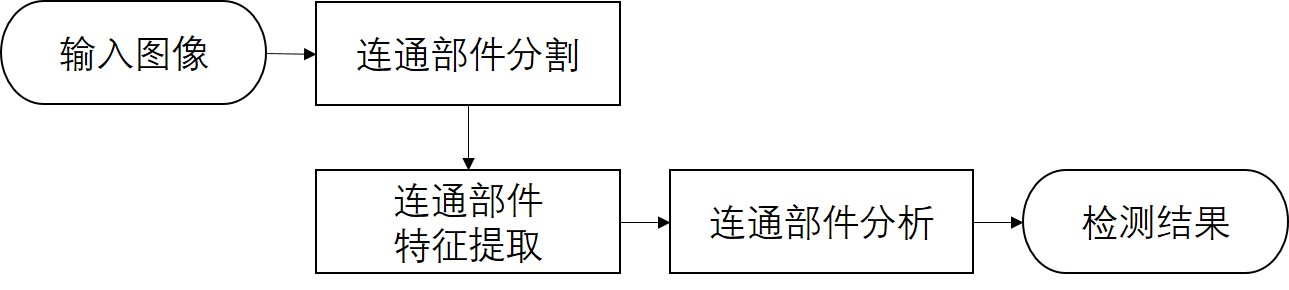
\includegraphics[width=\textwidth]{c2_cca_based.jpg}
    \caption{基于连通部件的文字检测方法的流程示例}
    \label{fig.c2_cca_based}
    \end{figure}

    如图\ref{fig.c2_cca_based}所示,这是一个典型的基于连通部件的检测方法的流程示例。在此类方法的流程中,通常首先会标记可能同属一个字符连通部件的像素,然后在分割连通部件的阶段通过把文字从背景中分离出来而得到候选的文字部件;接着在分析连通部件的阶段,首先提取笔画、几何、边缘及颜色等这些基于连通部件的特征,然后利用分类器来过滤掉非文字的部件;最后留下来的文字检测结果作为输出。

    Epshetein等\cite{Epshtein2010Detecting}提出用笔画宽度变换方法SWT来检测文字,促进了基于边缘(是连通部件中的一种)的文字检测算法的研究。这个方法根据图像里的文字笔画的宽度通常较为均一的属性,来过滤掉非文字边缘的像素。该方法首先利用Canny算子在场景文字图像的灰度图上求取图像中各目标的边缘,然后执行笔画宽度转换算法来计算笔画宽度图,其关键思路为:以边缘上的每个像素点为起始位置,沿该起始位置的梯度正负方向出发进行搜索,以找到梯度方向与起始位置点的方向近似相反的另一个边缘点,那么标记两像素点间的距离即为这个边缘的笔画宽度。在笔画宽度转换之后,再利用连通部件方法聚合起具有相近笔画宽度的像素点,以生成候选文字区域并方便后续的连通部件分析。最后使用启发性规则,例如欧拉数、宽高比等特征来过滤以得到真实文字区域。

    Yu等\cite{Yu2016Scene}是另一种基于边缘的文字检测方法。在该方法中,Yu等人提出了一种基于边缘重组、边缘滤波和多通道处理的自然场景图像文本检测与定位方法。为了从背景中分割出文本,在边缘分析过程中首先将边缘分割为一个个单独的边缘段,然后将这些边缘段重新组合到候选字符的连通部件上,并利用边缘滤波器滤除大部分的背景边缘,那么剩余下来的候选字符边缘将被链接到候选文本行上即得到定位结果。文中使用两种不同的分类器来过滤掉非文本行,并且为了更准确地进行分类,作者首先将提取到的特征存储在特征池中,然后利用SVM从特征池中选择最有效的特征来训练分类器。最后多通道用于确保文字检测查全率,而非极大抑制用来消除重复结果。   

    \begin{figure*}[!h]
    \centering
    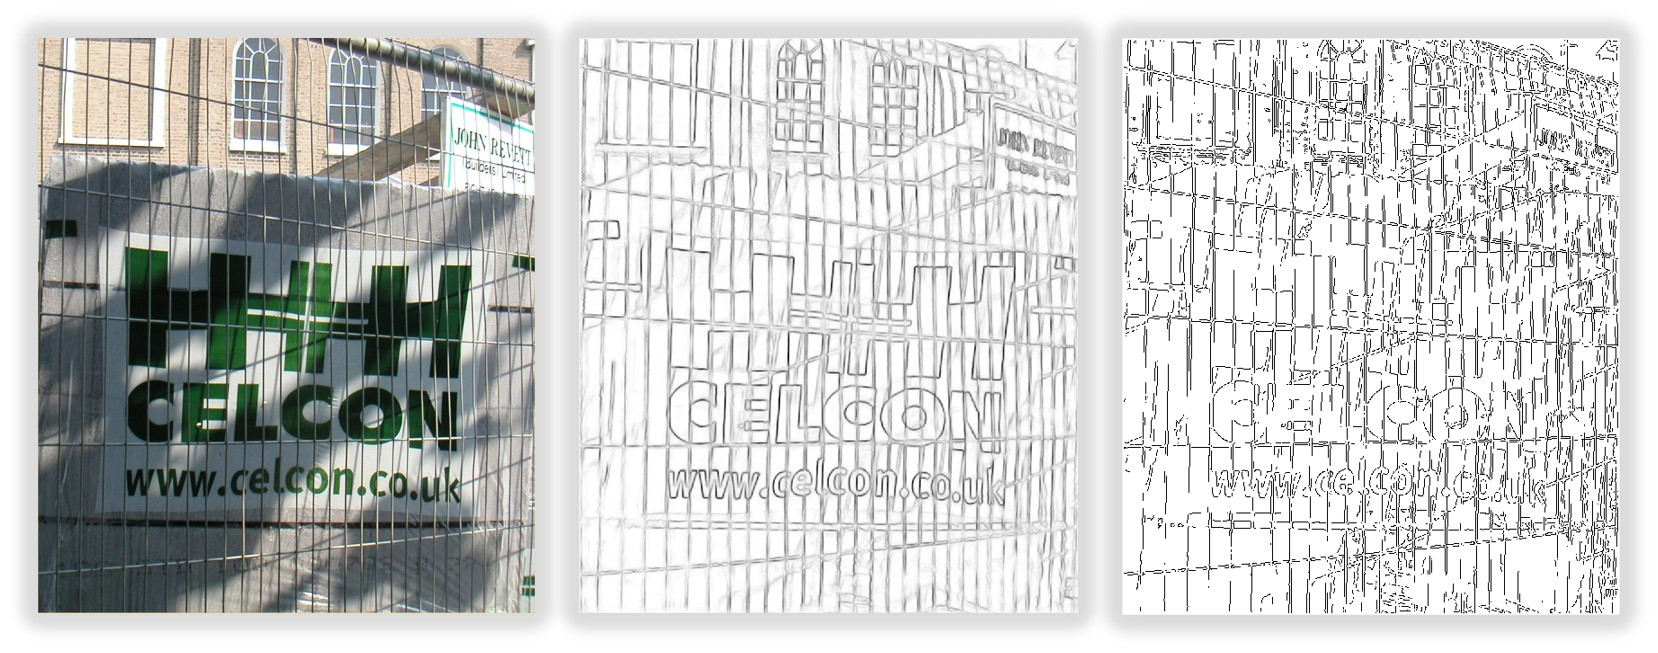
\includegraphics[width=\textwidth]{./figures/c2_sf_vs_canny.jpg}
    \begin{minipage}[t]{0.32\linewidth}
    \centerline{ \small (a) 原图}
    \end{minipage}
    \begin{minipage}[t]{0.32\linewidth}
    \centerline{ \small (b) 结构化边缘图}
    \end{minipage}
    \begin{minipage}[t]{0.32\linewidth}
    \centerline{ \small (a) Canny边缘}
    \end{minipage}
    \caption{基于结构化边缘检测算子和基于Canny边缘检测算子的结果对比}
    \label{fig.c2_sf_vs_canny}
    \end{figure*}

    上述基于连通部件的方法中,对文字边缘的检测大多使用Canny算子。而Dollar等\cite{Dollar2015Fast}提出一种新的结构化的边缘检测子。在这篇文章中,作者利用局部图像块中存在的结构来学习得到精确和高效的边缘检测器,并提出了一个应用于随机决策森林的结构化学习框架来预目标边缘掩码的问题。如图       \ref{fig.c2_sf_vs_canny}(b)所示,用结构化边缘检测子求取的边缘图要比Canny算子得到的如图\ref{fig.c2_sf_vs_canny}(c) 边缘图鲁棒且清晰得多。
    
    基于极值区域的方法是基于连通部件类方法中的另外一个比较经典和常见的文字检测方法。首先在文字检测方法中应用到最稳定极值区域MSER并获得显著的检测效果的是Neumann等\cite{Neumann2010A}提出的方法。而且Neumann在其后续研究如\cite{Neumann2011Text}里坚持依据MSER算法来提升文字检测算法的效果。MSER算法的原理如下:首先极值区域ER的概念即是区域外像素灰度值全部大于区域内部所有像素的区域,然后最稳定极值区域MSER便是在极值区域ER的基础上的图像分割方法。因为我们预设了候选文字目标的颜色均一并显著不同于背景,所以在对图像进行连续多个阈值的分割时,候选文字的目标区域面积会在一定阈值范围内呈现非常小的变化。
    
    \begin{figure*}[!h]
    \centering
    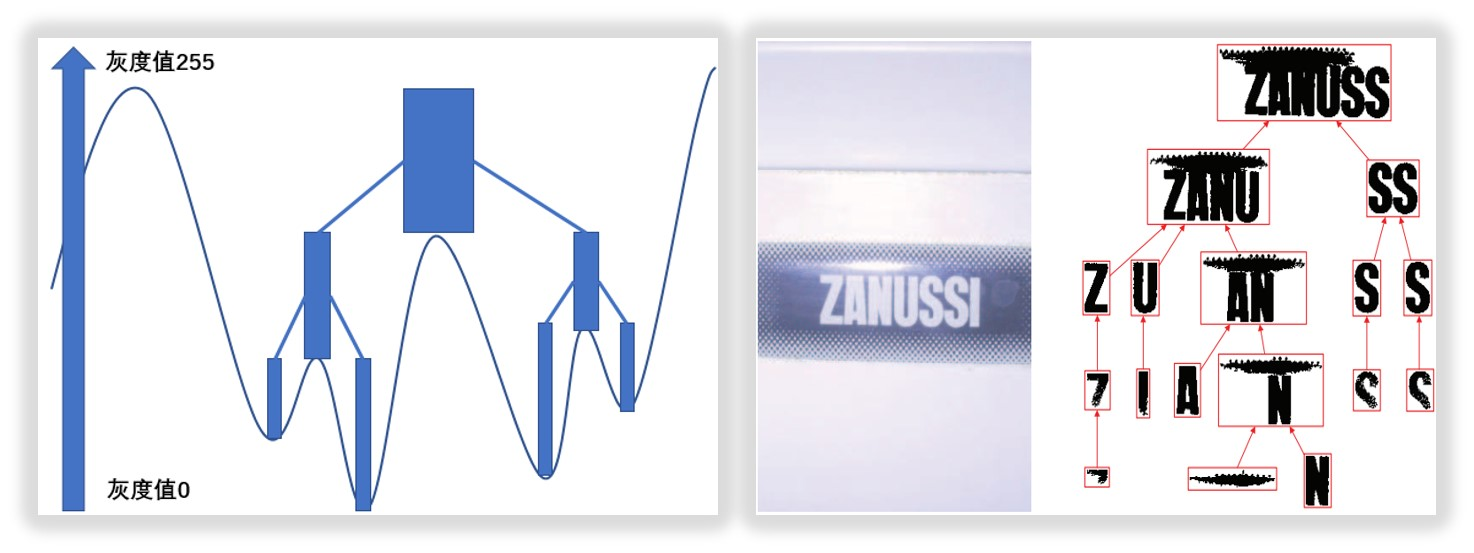
\includegraphics[width=\textwidth]{./figures/c2_er_tree.jpg}
    \begin{minipage}[t]{0.48\linewidth}
    \centerline{ \small (a) 分水岭算法}
    \end{minipage}
    \begin{minipage}[t]{0.48\linewidth}
    \centerline{ \small (b) 生成极值区域树}
    \end{minipage}
    \caption{生成极值区域树的示例图}
    \label{fig.c2_er_tree}
    \end{figure*}
    
    接下来Neumann又在方法\cite{Neumann2012Real}中反过来利用极值区域ER取代MSER以提取候选文字的连通部件,这是因为MSER对于一些模糊或光照过强的场景太敏感而漏检掉了候选文字部件,但ER却可以尽可能多的考虑到所有的连通部件,因为ER本来涵盖了MSER中所有的结果。生成ER树的过程如图\ref{fig.c2_er_tree}(b)所示,其原理类似于图\ref{fig.c2_er_tree}(a)的分水岭算法。在这类算法中,主要是利用ER树提取候选的文字部件,然后求取连通部件的空洞面积、欧拉数、水平交叉数目以及紧密度等特征,来训练SVM分类器以分类背景和文字。最后通过穷举搜索以将保留下来的连通部件排列成单词结果。

    \begin{table*}[!h]
    \centering
    \caption{基于连通部件的相关文字检测方法}
    \begin{tabular}{p{0.17\textwidth}|p{0.1\textwidth}| p{0.63\textwidth}}
    \hline
    作者 & 年份 & 方法概述 \\
    \hline
    Epshetein等\cite{Epshtein2010Detecting} & 2010年 & 候选文字筛选,笔画宽度转换SWT,文本行生成;\\
    Neumann等\cite{Neumann2011Text} & 2011年 &   最稳定极值区域MSER,穷举搜索\\
    Dollar等\cite{Dollar2015Fast} & 2015年 & 结构化边缘检测子,随机森林分类器 \\
    Yu等\cite{Yu2016Scene} & 2016年 & 文字的特征池,文字的边缘重组,以及SVM分类器 \\
    \hline
    \end{tabular}
    \label{tab.c2_connected_component_based}
    \end{table*}



    \section{本章小结}
    \esection{Brief Summary}


        % multiple1902 <multiple1902@gmail.com>
% intro.tex
% Copyright 2011~2012, multiple1902 (Weisi Dai)
% https://code.google.com/p/xjtuthesis/
%
% It is strongly recommended that you read documentations located at
%   http://code.google.com/p/xjtuthesis/wiki/Landing?tm=6
% in advance of your compilation if you have not read them before.
%
% This work may be distributed and/or modified under the
% conditions of the LaTeX Project Public License, either version 1.3
% of this license or (at your option) any later version.
% The latest version of this license is in
%   http://www.latex-project.org/lppl.txt
% and version 1.3 or later is part of all distributions of LaTeX
% version 2005/12/01 or later.
%
% This work has the LPPL maintenance status `maintained'。
%
% The Current Maintainer of this work is Weisi Dai。
%

\chapter{基于边缘骨架切割的文字检测方法}
\echapter{Text detection based on Skeleton-cut detector}
\label{sec.c3}

    边缘是一种可以很好地表征文字结构信息的特征。但是想要在自然场景图片的背景中分离出来文字边缘是一件极具困难的工作,其中最有挑战性的问题是如何解决边缘粘连(edge-adhesion)问题。针对这种边缘粘连问题,本文提出了一种基于边缘骨架切割的文字检测方法。

    \section{问题的提出}
    \esection{Questions Posed}

    基于区域和基于连通部件的文字检测方法各有优缺点。其中,基于区域方法的检测结构可在噪声环境中精准提取到文字,这是因为这些方法在图像上大多采用滑动窗进行细致的探索,并执行多尺度的处理来提取特征。但相应地就会导致分类窗口过多,计算量太大,对时间性能的要求也更高;而另一类方法的处理目标是连通部件,其数量相比滑动窗要更可控,因此处理时间大为缩短,并且其检测到的结果可直接应用到识别文字的阶段。但此类方法的问题是在曝光或低对比度环境中难以从背景中分离出连通区域,并且过于依赖图像分割算法的结果。如何对这两类方法折衷,以在保证精准的文字检测效果的同时还能达到较高的效率,是一个值得深入研究的问题。

    在基于区域的文字检测方法中主要有基于MSER和基于边缘的这两类主流方法。MSER类方法存在的问题有:当文字位于玻璃、浮雕等反光物体的表面时将无法作为极值区域被提取出来;采用ER树生成候选的文字区域会导致重复、嵌套和计算量过大等问题;用来过滤ER的启发式规则用到许多固定阈值。而基于边缘的方法对图像边缘提取的结果比较敏感,如果存在背景与文字边缘粘连问题,或不能完整提取文字边缘时,就很难进行后续的文字检测的分析,并造成漏检问题。针对上述的这些问题,一种解决办法便是利用文字自身的双边属性,而采用基于边缘的方法对此属性进行最佳的表征,然后再融合上MSER的方法来提取候选文字的感兴趣区域proposals,最后在这些proposals中进行单尺度滑动窗的变化并输入到CNN分类器中作分类。那么其中最关键的步骤就是解决背景与文字的边缘粘连问题,以提取出完整的文字边缘。

    依据以上提出的问题及对其的分析,本文提出了一种基于边缘骨架切割的文字检测方法。首先求取场景文字图片的边缘骨架图,并在其上利用8 连通域分析方法找到文字边缘和背景边缘的粘连点。然后自适应地断开这些粘连点,并将分离开来候选文字边缘骨架段输入到两阶段的CNN分类器中作文字与非文字的判别。最后提出一种结合MSER的局部迭代优化算法来提高文字检测的准确度。

    \section{方法原理与步骤}
    \esection{Principle and Summary of The Method}

    基于边缘骨架切割的文字检测子的具体流程如图\ref{fig.c3_overview} 所示。首先对于输入的场景文字图片,利用结构化边缘检测方法\cite{Dollar2015Fast} 得到输入图片的结构化边缘响应图,如图\ref{fig.c3_overview}(b) 所示。然后基于一系列像素强度值阈值,对边缘响应图进行分割,得到相应的二值化边缘图。接着在每个二值边缘图上,通过细化操作得到其边缘骨架图,如图\ref{fig.c3_overview}(c) 所示。图中的红色结点是在边缘骨架上,通过8 领域内像素点分析所找到的边缘骨架结点。而文字边缘与背景间的粘连点,就存在于这些边缘骨架结点中。
    为了将文字边缘从背景杂质中切割出来,需要切割开这些边缘骨架结点,以解决文字边缘的粘连问题。而由不同的二值边缘图所生成的边缘骨架图上的结点是不同的。因此选择合适的边缘骨架图上的结点进行切割,是解决文字边缘粘连问题的核心步骤。

    \begin{figure*}[!h]
    \centering
    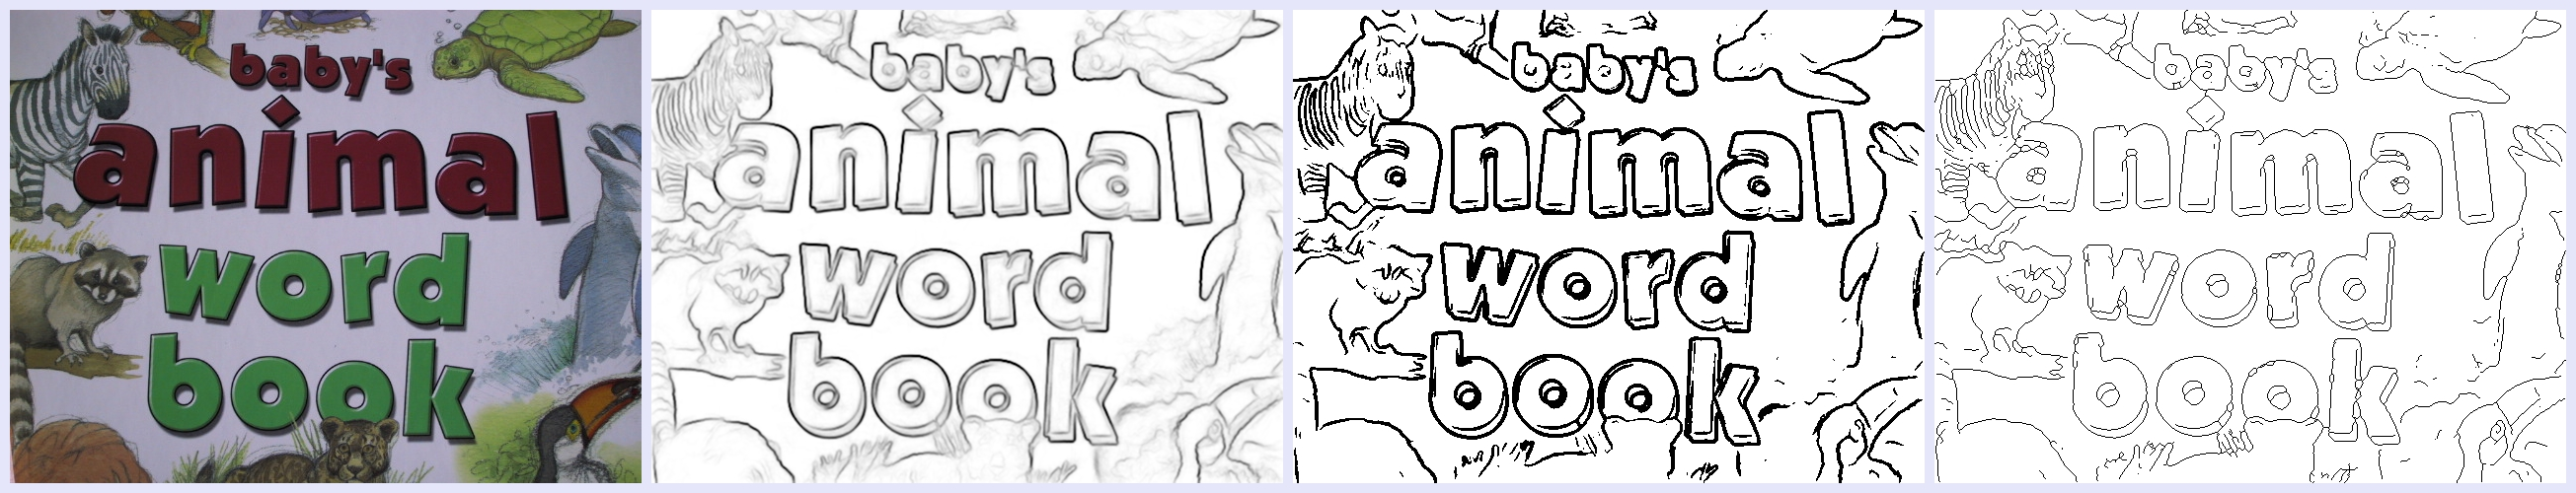
\includegraphics[width=\textwidth]{./figures/c3_overview_1.jpg}
    \begin{minipage}[t]{0.22\linewidth}
    \centerline{ \small (a) 输入场景文字图}
    \end{minipage}
    \begin{minipage}[t]{0.22\linewidth}
    \centerline{ \small (b) 边缘响应}
    \end{minipage}
    \begin{minipage}[t]{0.22\linewidth}
    \centerline{ \small (c) 边缘二值图}
    \end{minipage}
    \begin{minipage}[t]{0.22\linewidth}
    \centerline{ \small (d) 边缘骨架}
    \end{minipage}
    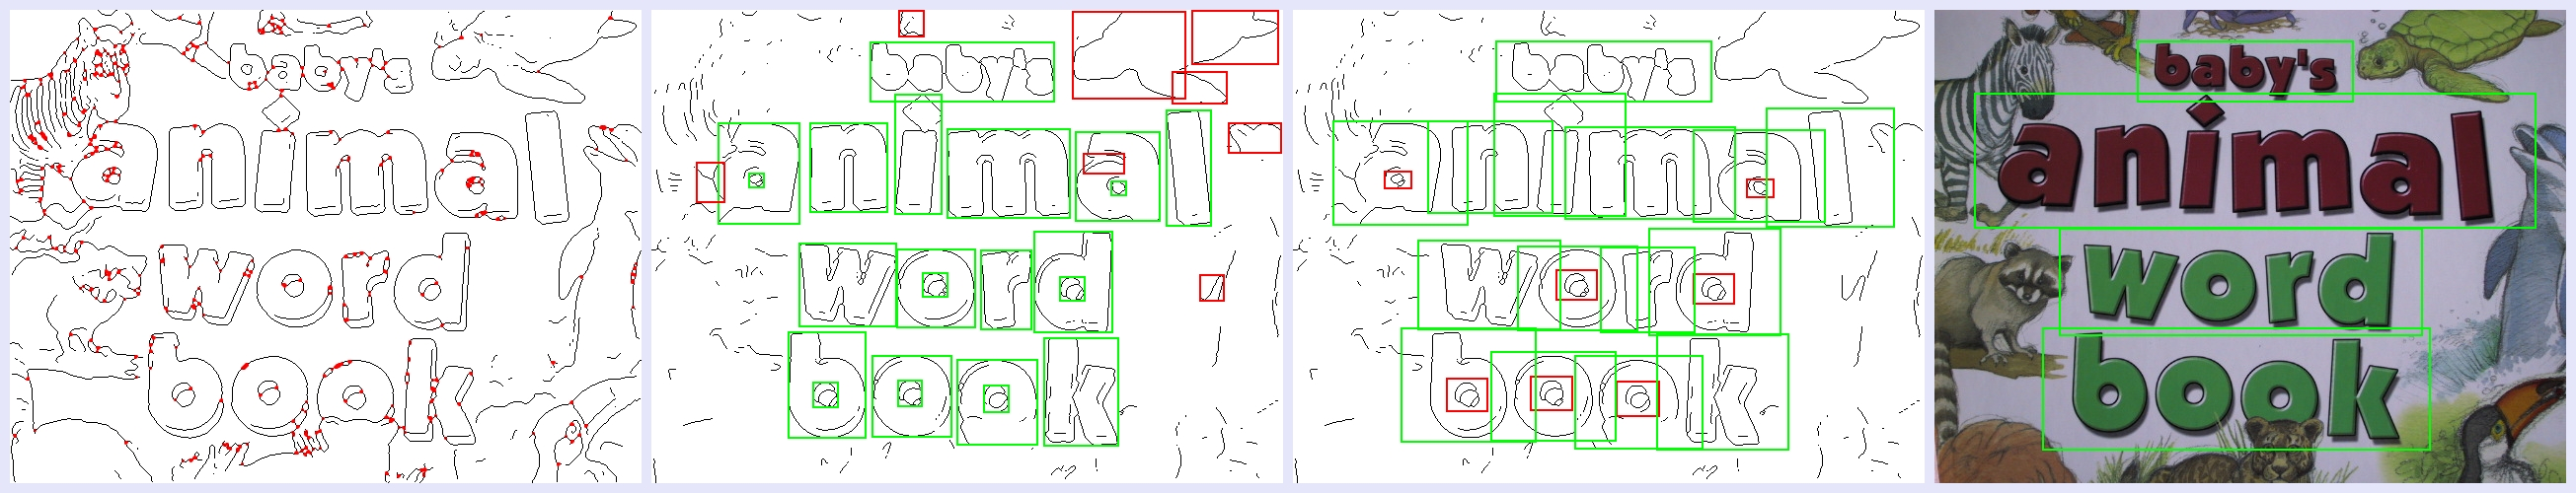
\includegraphics[width=\textwidth]{./figures/c3_overview_2.jpg}
    \begin{minipage}[t]{0.22\linewidth}
    \centerline{ \small (e) 边缘骨架切割}
    \end{minipage}
    \begin{minipage}[t]{0.22\linewidth}
    \centerline{ \small (f) 非文字骨架的滤除}
    \end{minipage}
    \begin{minipage}[t]{0.22\linewidth}
    \centerline{ \small (g) 文本行生成}
    \end{minipage}
    \begin{minipage}[t]{0.22\linewidth}
    \centerline{ \small (h) 文字粗略定位结果}
    \end{minipage}
    \caption{基于边缘骨架切割的文字检测方法的流程图}
    \label{fig.c3_overview}
    \end{figure*}

    这里通过实验观察可知,那些分割阈值较低所得的二值边缘图所生成的边缘骨架较为杂乱,更可能是无效的边缘骨架,如图\ref{fig.c3_select_skeleton}(a) 所示。
    因此这里采用欧拉数计算,来从一系列边缘骨架图中选择出最合适的边缘骨架图,欧拉数的计算过程如图\ref{fig.c3_select_skeleton}(b) 所示。在边缘骨架图中,所有的候选边缘骨架都要经过形态学滤除,以过滤掉大部分明显不是文字的边缘骨架。该滤除过程如图\ref{fig.c3_overview}(c) 到图\ref{fig.c3_overview}(d) 的变化所示。紧接着,剩余的不易区分的非文字边缘骨架,可通过基于CNN 的分类器来进一步滤除。该滤除过程如图\ref{fig.c3_overview}(d) 到图\ref{fig.c3_overview}(e) 所示,红色框中包含的不易区分的非文字边缘骨架,可通过CNN 分类器去除掉。最后如图\ref{fig.c3_overview}(f) 所示,基于非极大值抑制和文本行聚集操作,得到粗略的文本行定位结果。

    \section{文字骨架的提取与切割}
    \esection{Text skeleton's extraction and cutting}

        \subsection{文字骨架的生成}
        \esubsection{Text skeleton's construction}
        \label{sec.c3_skeleton}

        %一系列分割阈值,得到不同的二值边缘图,并生成相应的边缘骨架图;低分割阈值的二值图所生成骨架图较为杂乱,不适合用于后续的边缘骨架切割步骤;这部分内容在supplement 上有,将其作图写在skeleton 的生成一节中。

        在输入的场景文字图像上,通过结构化边缘检测子\cite{Dollar2015Fast} 得到了图像的结构化边缘响应图。边缘响应图并不是二值图,其每个位置上的像素点的值代表的是该像素点属于边缘的概率。如图\ref{fig.c3_overview}(b) 所示,某位置的像素点的值越大,图中该位置的像素点的颜色就越深,说明该位置的像素点越可能位于一条边缘之上。既然边缘响应图是每个位置像素点的值都不尽相同的概率图,为了便于观察,用图\ref{fig.c3_response_to_map} 第一行的三维图展示其概率响应。然后按照一系列像素灰度值阈值,对边缘响应图进行分割,得到相应阈值下的二值边缘图。这些二值边缘图如图\ref{fig.c3_response_to_map} 中第二行所示。

        从图\ref{fig.c3_response_to_map} 中可以看出,当分割阈值较小时,从边缘响应图上分割得到的二值边缘图较为清晰,但存在大量非文字的边缘,导致文字边缘与背景的粘连问题较为严重。而当分割阈值较大时,从边缘响应图上分割得到的二值边缘图中,大部分非文字的边缘已经被略去,而文字边缘相对而言被较为完整的保留下来,使得文字边缘的粘连问题得到缓解。但同时,大阈值分割下的二值边缘图较为模糊和残缺,边缘时有断裂现象,不利于后续的边缘分析与处理。

        \begin{figure*}[!h]
        \centering
        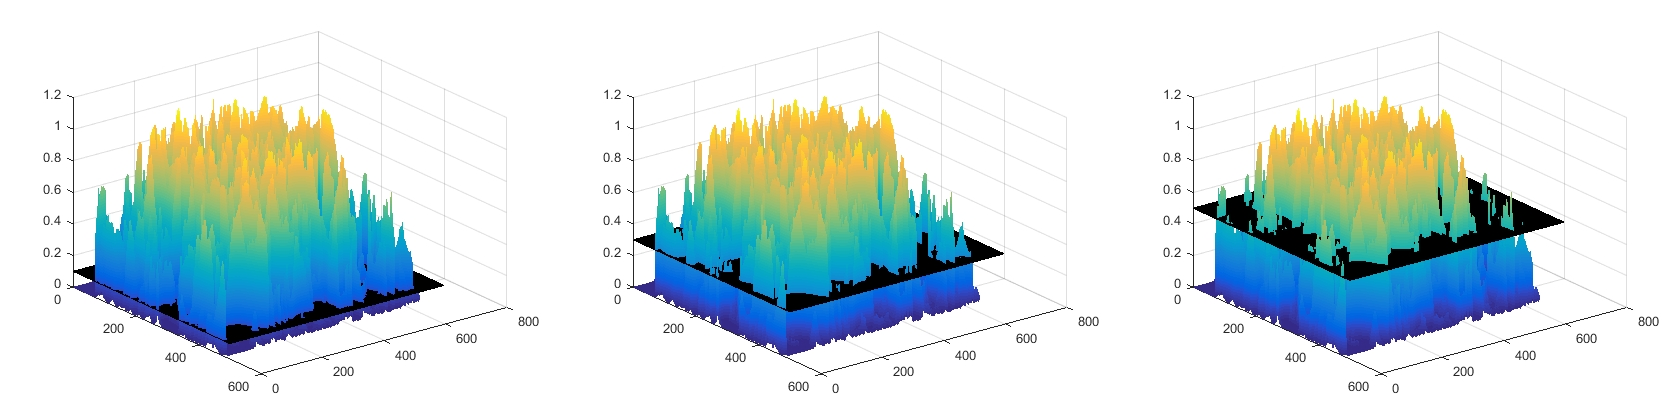
\includegraphics[width=\textwidth]{./figures/c3_edge_response.jpg}
        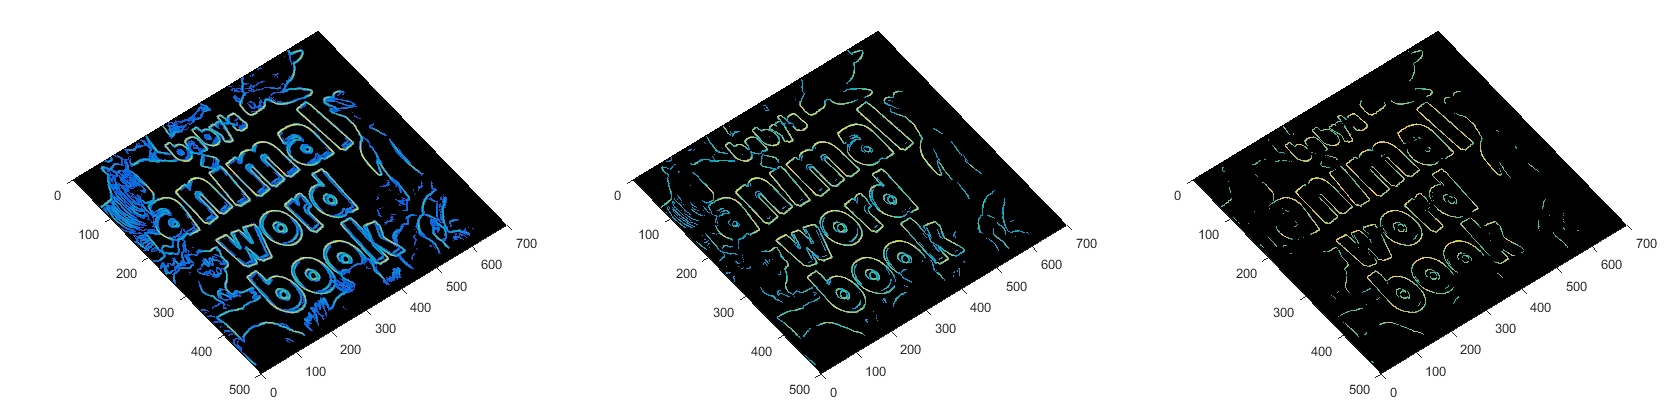
\includegraphics[width=\textwidth]{./figures/c3_edge_map.jpg}
        \begin{minipage}[t]{0.32\linewidth}
        \centerline{ \small (a) 阈值 $t = 0.1$}
        \end{minipage}
        \begin{minipage}[t]{0.32\linewidth}
        \centerline{ \small (b) 阈值 $t = 0.3$}
        \end{minipage}
        \begin{minipage}[t]{0.32\linewidth}
        \centerline{ \small (c) 阈值 $t = 0.5$}
        \end{minipage}
        \caption{在边缘响应图上通过一系列的分割阈值得到相应的边缘二值图}
        \label{fig.c3_response_to_map}
        \end{figure*}

        因此,分割阈值不同,从边缘响应图上分割得到的二值边缘图也不同。较高阈值下的边缘图保留了更多的边缘信息,但更难区别文字与非文字边缘。较低阈值的边缘图去除了非文字边缘信息,但边缘更不清晰。不同于Canny 算子\cite{Ding2001On} 等固定阈值的边缘二值图检测方法,本文采用递增的分割阈值从边缘响应图中得到一系列候选边缘二值图,然后从中自适应地选择出最合适的二值边缘图进行后续处理。自适应选择最优二值边缘图的内容会在\ref{sec.c3_skeleton_cut} 节中详细阐述。

        接下来利用8连通区域细化方法\cite{Lam2002Thinning} 在二值边缘图上提取边缘的骨架线。该细化方法会一直重复迭代操作,直到图像不再发生变化。每次迭代操作包含2个子迭代操作:在第1个子迭代操作中,当且仅当条件 $G_1$, $G_2$ 和 $G_3$ 全部满足时,二值边缘上的像素点$p$ 将被消除。而在第2个子迭代操作中,当且仅当条件$G_1$, $G_2$ 和 $G_3$$'$ 全部满足时,二值边缘上的像素点$p$ 将被消除。这些细化操作的条件如下所示:

        1)条件$G_1: X_H(p)=1$

        其中,$X_H(p)=\sum\limits_{i=1}^4b_i$,而
        $b_i=\left\{
        \begin{array}{cl}
        1, &  if \ x_{2i-1}=0 \; and \; (x_{2i}=1 \; or \; x_{2i+1}=1)\\
        0, &  otherwise.
        \end{array}
        \right.$

        2)条件$G_2: 2\le \left\{n_1(p),n_2(p)\right\} \le3$

        其中,$n_1(p)=\sum\limits_{k=1}^4x_{2k-1}\lor x_{2k}$,并且
        $n_2(p)=\sum\limits_{k=1}^4x_{2k} \lor x_{2k+1}$

        3)条件$G_3: (x_2 \lor x_3 \lor \overline{x}_8) \land x_1=0$

        4)条件$G_3$$'$$: (x_6 \lor x_7 \lor \overline{x}_4) \land x_5=0$

        细化方法将重复迭代操作,直到提取出的边缘的骨架图不再变化为止。因此候选文字骨架的生成步骤如图\ref{fig.c3_skeleton} 所示:首先利用结构化边缘检测子在输入的场景文字图像中计算得到结构化边缘响应,然后通过一系列分割阈值获得相应的二值边缘图,最后通过8 连通区域细化方法得到边缘骨架图,即宽度为1 个像素宽的边缘骨架线,如图\ref{fig.c3_skeleton}(d) 中的1 个像素宽的黑色细线所示。

        \begin{figure*}[!h]
        \centering
        
\includegraphics[width=\textwidth]{./figures/c3_skeleton.jpg}
        \begin{minipage}[t]{0.24\linewidth}
        \centerline{\small (a)原图}
        \end{minipage}
        \begin{minipage}[t]{0.24\linewidth}
        \centerline{\small (b)边缘响应}
        \end{minipage}
        \begin{minipage}[t]{0.24\linewidth}
        \centerline{\small(c) 边缘二值图}
        \end{minipage}
        \begin{minipage}[t]{0.24\linewidth}
        \centerline{\small (d)边缘骨架图}
        \end{minipage}
        \caption{文字边缘骨架生成的流程图}
        \label{fig.c3_skeleton}
        \end{figure*}

        \subsection{文字骨架粘连点的检测和切割}
        \esubsection{Text adhesion-junctions' detection and cutting}
        \label{sec.c3_skeleton_cut}

        生成边缘骨架图后,就可以通过8 连通区域的像素点数分析来检测边缘骨架粘连点。检测边缘骨架粘连点$J$ 的公式如下所示:

        \begin{equation}
        J=\left\{ p|n(p)=\sum_{k=1}^8x_k>t \right\},
        \label{eq:c3_junctions}
        \end{equation}

        在公式\ref{eq:c3_junctions} 中,$n_p$ 是像素点$p$ 的8 连通区域内像素点的数目之和,而$t$ 是用来提取粘连点的像素点数目阈值。通过实验观察,令$t = 3$ 能检测到数目合适的候选边缘骨架粘连点,如图\ref{fig.c3_skeleton} 中的红色结点所示。

        在\ref{sec.c3_skeleton} 节中已经阐述,对于边缘响应图,利用不同的分割阈值可以得到相应的二值边缘图。而且分割阈值较大时,二值边缘清晰但粘连问题严重,阈值较小时非文字边缘大部分被消除但是文字边缘也出现断裂问题。因此选择合适的二值边缘图,使得既不会在图中出现过多的背景边缘,又能提供清晰的边缘信息,对后续解决边缘粘连问题至关重要。而观察由二值边缘图所生成的边缘骨架图的形态,就是一种判断所选边缘图是否合适的方式。

        \begin{figure*}[!h]
        \centering
        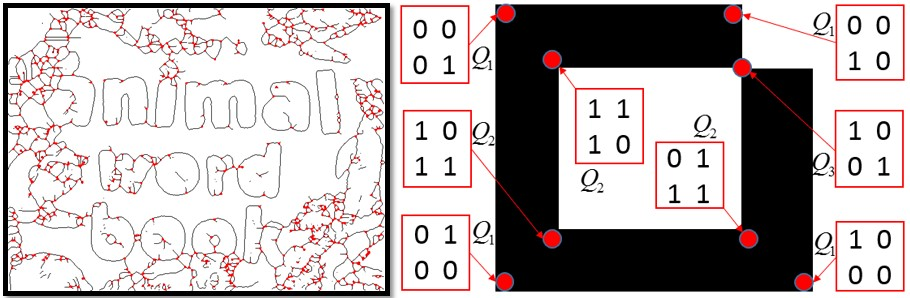
\includegraphics[width=\textwidth]{./figures/c3_select_skeleton.jpg}
        \begin{minipage}[t]{0.48\linewidth}
        \centerline{\small (a)无效的边缘骨架图}
        \end{minipage}
        \begin{minipage}[t]{0.48\linewidth}
        \centerline{\small (b)在边缘骨架图上计算欧拉数}
        \end{minipage}
        \caption{通过欧拉数的计算,选择出最合适的边缘骨架图}
        \label{fig.c3_select_skeleton}
        \end{figure*}

        如图\ref{fig.c3_select_skeleton}(a) 所示,当分割阈值偏小时,从边缘响应图上分割得到的二值边缘图中混有过多的非文字边缘信息,因此通过细化操作所得的边缘骨架图十分杂乱无序,不能作为解决边缘粘连问题的有效信息。在这种混乱的边缘骨架图上检测到的候选边缘骨架粘连点,数目特别多且分布杂乱。因此,检测到的候选边缘骨架粘连点的数目,在一定程度上可以指示所选二值边缘图和相应的边缘骨架图的合理程度。除此之外,还可以通过对生成的边缘骨架图计算欧拉数,来避免选择不合适的边缘骨架图。

        \begin{figure*}[!h]
        \centering
        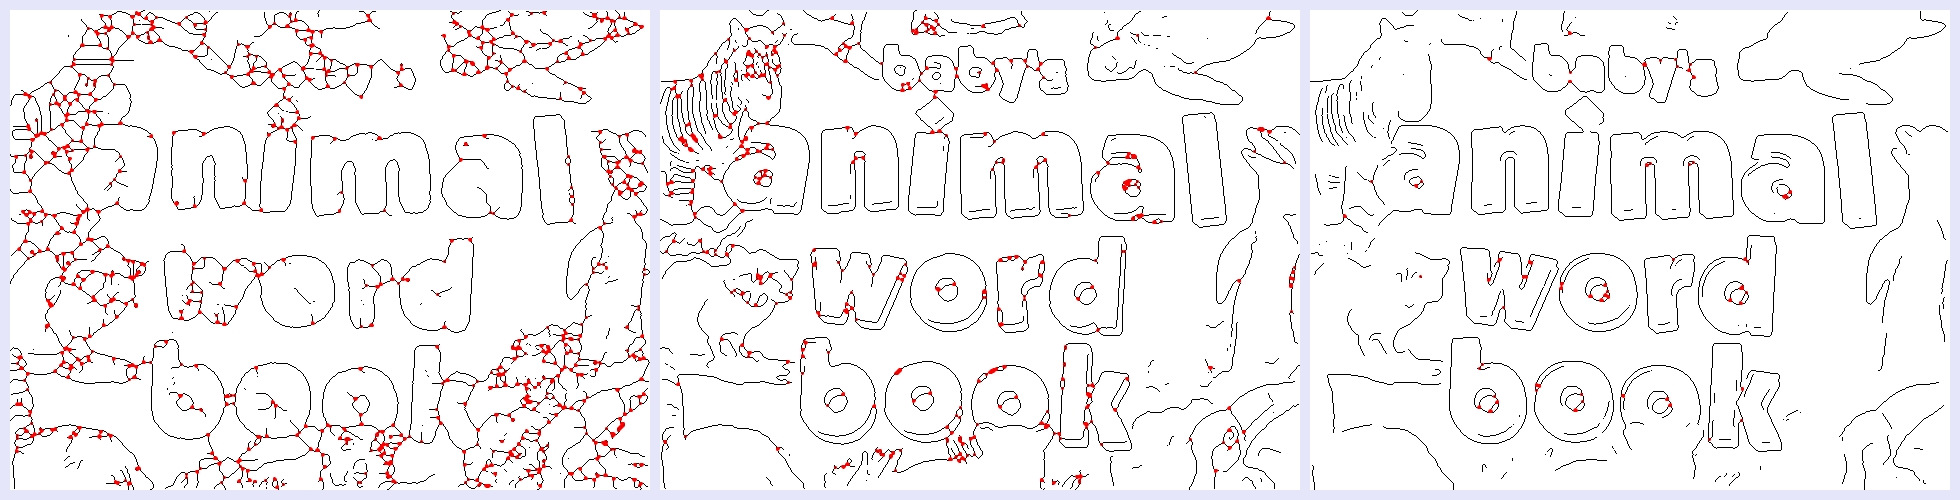
\includegraphics[width=\textwidth]{./figures/c3_compare_skeleton.jpg}
        \caption{不同的边缘骨架图的连通区域数目稳定,但孔洞数目变化剧烈}
        \label{fig.c3_compare_skeleton}
        \end{figure*}

        欧拉数是二值图像的拓扑特征,其数值是连通区域数目与孔洞数目的差值。由不同的二值边缘图所生成的边缘骨架图,它们的连通区域数目比较稳定,但是孔洞数目的变化很剧烈。如图\ref{fig.c3_compare_skeleton} 所示,过低或过高的分割阈值下的二值边缘图所生成的边缘骨架图的孔洞数与连通区域的数目的差距很大,而正常分割阈值下的边缘骨架图中孔洞数目和连通区域数目的差值则保持在合理范围内。

        1种简单且有效的计算欧拉数的方法是计算$2*2$ 像素模式的数目,这些像素模式的类型存在以下几类:

        $Q_1 = \left\{
        \quad
        \begin{matrix} 1 & 0 \\ 0 & 0 \end{matrix}\quad,\quad
        \begin{matrix} 0 & 1 \\ 0 & 0 \end{matrix}\quad,\quad
        \begin{matrix} 0 & 0 \\ 0 & 1 \end{matrix}\quad,\quad
        \begin{matrix} 0 & 0 \\ 1 & 0 \end{matrix}
        \quad
        \right\}$

        $Q_2 = \left\{
        \quad
        \begin{matrix} 0 & 1 \\ 1 & 1 \end{matrix}\quad,\quad
        \begin{matrix} 1 & 0 \\ 1 & 1 \end{matrix}\quad,\quad
        \begin{matrix} 1 & 1 \\ 1 & 0 \end{matrix}\quad,\quad
        \begin{matrix} 1 & 1 \\ 0 & 1 \end{matrix}
        \quad
        \right\}$

        $Q_3 = \left\{
        \quad
        \begin{matrix} 0 & 1 \\ 1 & 0 \end{matrix}\quad,\quad
        \begin{matrix} 1 & 0 \\ 0 & 1
        \end{matrix}
        \quad
        \right\}$

        其中,$Q_1$为外角点,$Q_2$ 为内角点,$Q_3$ 为交叉点,这些角点在边缘骨架上的位置如图\ref{fig.c3_select_skeleton}(b) 所示。那么欧拉数目的计算可由公式\ref{eq:c3_euler_number} 得到:

        \begin{equation}
        \eta=\frac{n(Q_1)-n(Q_2)+2n(Q_3)}{4},
        \label{eq:c3_euler_number}
        \end{equation}

        接下来,只有欧拉数和粘连点数最合适的边缘骨架图被保留下来,其它的边缘骨架图全部被删去。通过上述方式选择出来的边缘骨架图,既避免了过高分割阈值下的边缘图所可能生成的碎片和断裂化的边缘骨架,又避免了过低分隔阈值时可能生成的孔洞过多的杂乱边缘骨架,且因为删去了绝大多数无效的候选边缘骨架,而节省了计算量和时间。最后,将最合适的边缘骨架图上的粘连点消除掉,即可以将候选文字边缘骨架从背景中分离出来,以此来解决边缘粘连问题。

    \section{非文字骨架的滤除}
    \esection{Non-text skeleton's filtering}

    在\ref{sec.c3_skeleton}节中,我们论述了边缘骨架的生成方法,而在\ref{sec.c3_skeleton_cut} 节阐明了从背景中分隔出候选文字边缘骨架的具体步骤。目前,所有候选文字边缘骨架与非文字的边缘骨架之间的粘连点已经断裂开来,因此边缘粘连问题被解决了。但是在这些候选的边缘骨架中,还混杂有一些非文字的边缘骨架,需要被分类判别出来并清楚掉。所以在本节,提出1 个两阶段的文字边缘骨架分类方法,用以滤除掉混杂在文字边缘骨架中的非文字边缘骨架杂质。

        \subsection{形态学滤除}
        \esubsection{Morphological filtering}

        第1阶段的分类方法是形态学滤除。首先,从图\ref{fig.c3_compare_skeleton}(a) 和图\ref{fig.c3_compare_skeleton}(b) 的对比中,我们可以分析出文字边缘骨架和非文字边缘骨架之间在形态上的不同:背景边缘骨架比较直且分散,而文字边缘骨架则相对而言弯曲且聚合在一起。基于这一观察,大量的非文字边缘骨架就可以通过一些形态学的限制来过滤掉。

        \begin{figure*}[!h]
        \centering
        
\includegraphics[width=\textwidth]{c3_skeleton_samples.jpg}
        \begin{minipage}[t]{0.48\linewidth}
        \centerline{\small (a)文字边缘骨架}
        \end{minipage}
        \begin{minipage}[t]{0.48\linewidth}
        \centerline{\small (b)非文字边缘骨架}
        \end{minipage}
        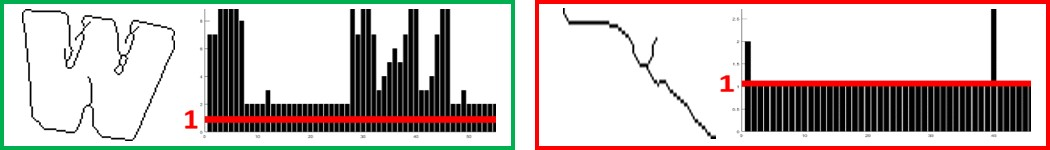
\includegraphics[width=\textwidth]{c3_concentration_ratio.jpg}
        \centerline{\small (c) 文字通常比非文字骨架具有更高的聚合度}
        \caption{文字与非文字边缘骨架的聚合度的比较} \label{fig.c3_concentration_ratio}
        \end{figure*}

        这些常用的形态学的限制包括:宽高比,离心率,欧拉数,同时在区域和其最小凸多边形中的像素比例,等等。而在本文中,针对文字边缘骨架和非文字边缘骨架的不同,提出一种简单但高效的形态学限制,即边缘骨架的聚合程度。假设给定边缘骨架$skel$,求取该边缘骨架的聚合度的方式如公式\ref{eq:c3_concentration_ratio} 所示:

        \begin{equation}
        C(skel)=\frac{length(skel_{ol})}{length(skel)},
        \label{eq:c3_concentration_ratio}
        \end{equation}

        其中,$skel_{ol}$是边缘骨架$skel$ 重叠的部分,即$skel_{ol}=skel(sum_{ver}(skel)>1)$。 而$Sum_{ver}(skel)$ 是按竖直方向将边缘骨架$skel$ 累加起来,如图\ref{fig.c3_concentration_ratio}(c) 所示:红线代表竖直方向累加像素点的个数为1 的阈值线,那么超过红线的位部分,表示该位置上存在重叠的边缘骨架$skel_{ol}$,即在$skel_{ol}$ 中 $Sum_{ver}(skel)>1$。 通过对图\ref{fig.c3_concentration_ratio}(c) 的观察,文字边缘骨架绝大部分都是重叠的,也就是$skel_{ol}$ 的长度占$skel$ 长度的比率$C(skel)$ 较大,因此较大的比率$C(skel)$ 表征了文字边缘骨架具有更高的聚合度。与此同时,观察发现非文字边缘骨架只有很小一部分是重叠的,即$skel_{ol}$ 的长度占$skel$ 长度的比率$C(skel)$ 很小,所以小$C(skel)$ 表征了非文字边缘骨架的聚合度更小。

        通过在第1阶段分类过程中,采用上述的这些简单的形态学限制,包括本文新提出的针对文字边缘骨架特征的聚合度限制,绝大多数非文字的边缘骨架就可以被高效的过滤掉。但是可能存在一些与文字边缘骨架极为相近的非文字边缘骨架没有在形态学过滤阶段被排除。那么这些被遗漏的非文字边缘骨架,就将在后续的第2 阶段分类过程中进行过滤。

        \subsection{基于卷积神经网络的滤除}
        \esubsection{convolutional neural network-based filtering}

        第2阶段的分类过程是更为精细的分类操作。受Wang 等\cite{Wang2012End} 提出的利用卷积神经网络(CNN) 作端对端文字识别方法的启发,在精细分类阶段我们提出一种基于CNN 的文字边缘骨架分类器,用于滤除掉遗漏下来的非文字边缘骨架。这个基于CNN 的边缘骨架分类器的架构如图\ref{fig.c3_cnn}所示,其网络结构是由2 个卷积层,分别后接2 个池化层,最后连1 个全连接层构成。其中第1 个卷积层有$n_1 = 64$ 个卷积模板,第2 个卷积层有$n_2 = 128$ 个卷积模板。全连接层后接2 个类别,分别为文字边缘和非文字边缘类别。2 类中置信度更高的类别即为分类判别结果。

        \begin{figure*}[!h]
        \centering
        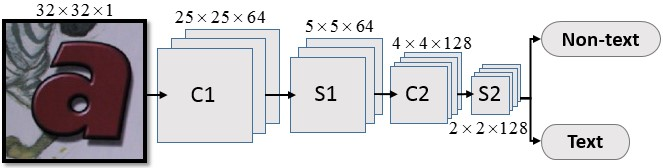
\includegraphics[width=\textwidth]{c3_cnn.jpg}
        \caption{单尺度卷积神经网络分类器的架构} \label{fig.c3_cnn}
        \end{figure*}

        这个CNN网络结构的输入是例如图\ref{fig.c3_cnn} 中最左边的小图块。这些小图块,是由经过第1阶段分类后被判别为候选文字边缘骨架的包围框,在原图上截取下来的小图块组成。在训练阶段,将这些图块的大小调整成$32 \times 32$ 个像素大小的训练样本,输入到CNN 网络中。然后在第1 个卷积层中,得到$25 \times 25 \times n_1$个卷积响应。接着在平均池化层,将响应的维度缩减到$5 \times 5 \times n_1$。 类似地,经过第2个卷积层和池化层处理后,得到$2 \times 2\times n_1$ 的响应,并全连接到最后的分类层。训练网络时用squared hinge loss 作为损失函数。

        而在测试阶段,首先用基于Skeleton-cut 的文字边缘骨架检测子来生成候选的文字边缘骨架集合$P$,以及这些文字边缘骨架相对应的包围框集合$B$。与Wang 等\cite{Wang2012End} 方法中利用滑动窗在原图的多尺度金字塔图像中扫描全图来计算卷积和池化响应不同,本文中要进行卷积处理的图块既不需要扫描全图,也不用因为考虑多尺度文字而在原图的多尺度金字塔图像上扫过滑动窗。本文只要对候选文字边缘骨架集合$B$ 中的每个边缘骨架的图块作分类判别即可,并且对这些图块只需作单尺度$s = height(B)$ 的变化。因此相比较过去的基于滑动窗的CNN分类判别器而言,本文中利用CNN 进行文字与非文字边缘骨架分类的方法要更为高效和省时。

        最终,经过2层卷积和池化的响应输入到SVM 分类器,由此得到候选文字边缘骨架集合$P$ 中每个候选边缘骨架$p$ 的分类分数。这其中,具有较低文字分类置信度的候选文字边缘骨架将会被删除。那么经过第2阶段过滤后,保留下来的文字边缘骨架包围框的集合$B$ 就是基于边缘骨架切割的文字检测方法的结果。集合$B$ 中的每个文字边缘骨架包围框都有自己相应的分类置信度成绩$C$。

    \section{文本行的局部迭代优化}
    \esection{Text line's iteratively local refinement}

    本文上述所提出的基于边缘骨架切割的检测方法和2 阶段分类判别方法可以获得较高的文字检测查全率,但是文字检测结果同真实结果值(ground truth)之间的重叠率还是不满足期望。为了达到文字检测过程中的紧凑性(compactness) 标准,我们通过下面的算法\ref{alg:c3_iter_local_refine} 来调整文字检测包围框,使其更靠近文字的真实位置:

    \begin{algorithm}[!h]
	\renewcommand{\algorithmicrequire}{\textbf{输入:}}
	\renewcommand{\algorithmicensure}{\textbf{输出:}}
	\caption{文本行的局部迭代优化算法}
	\label{alg:c3_iter_local_refine}
	\begin{algorithmic}[1]
		\REQUIRE 候选文字边缘骨架的包围框集合 $B$, 以及求取的MSER 集合 $M$
		\ENSURE 经过局部迭代优化操作,对定位调整后的包围框集合 $R$
		\STATE 将MSER集合$M$按照位置分成2 类:强MSER 子集合$S$,是指包含在$B$ 边界内部的MSER 集合;弱MSER 子集合$W$ ,是指位于$B$ 边界之外的MSER 集合
        \FOR {$b \in B$}
        \STATE //本算法的目的是:在文本行方向上,将$b$ 调整为$b_{exp}$
        \STATE 计算位于$b$中的MSER$S$ 的特征均值$ms$
		\REPEAT
        \STATE $ws:=\left\{ w \in W |\,ol(b_{exp},w)>T_{ol}, | yc_{ms}-yc_w|<T_{yc} \right\}$
        \STATE $rs:=\left\{ w \in ws |\,Dist_{h,w,sw,c}(ms,w)<T_{h,w,sw,c} \right\}$
        \STATE $S:=S\cup rs,W:=W / rs$
        \UNTIL{$rs=\varnothing$}
        \STATE $R:=B \cap S$
        \ENDFOR
	\end{algorithmic}
    \end{algorithm}

    其中,$Dist_f(s,w)$指的是$s_f$ 和$w_f$ 之间归一化的$L2$ 距离。而$f$ 是候选MSER 的特征,这些特征包含:$sw$ 是笔划宽度,$c$ 是HSV 和灰度的颜色通道,$h,w$是候选MSER的高度和宽度;$yc$ 是候选MSER 在y 坐标轴上的中心坐标;另外函数$ol$用以计算2 个候选MSER 的包围框之间的重叠率;而$T$ 是经过实验计算得出的经验阈值。

    \begin{figure*}[!h]
    \centering
    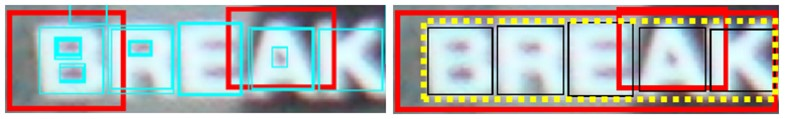
\includegraphics[width=\textwidth]{c3_iter_local_refine.jpg} \caption{局部迭代优化的效果示例}
    \label{fig.c3_iter_local_refine}
    \end{figure*}

    利用局部迭代优化方法来矫正文本行的实验效果如图\ref{fig.c3_iter_local_refine} 所示:图中左边的是未经过局部迭代优化前的文字检测结果,其中用红色矩形框标注的是用基于边缘骨架切割的检测子提取出的候选文字,用蓝色矩形框标注的是用MSER 提出的候选文字;而图中右边的是经过局部迭代优化后得到的文字检测结果,可看出通过算法\ref{alg:c3_iter_local_refine} 将基于边缘骨架切割的文字检测子和基于MSER 的检测方法结合起来,从而追回那些因图像模糊而未被检测到的候选文字。通过文本行局部迭代优化后得到的最终检测结果如图\ref{fig.c3_iter_local_refine} 中右图内的黄色虚线包围框所示,可见包围框的查全率以及同真实结果值之间的重叠率都得到了极大提升。

    \section{实验和结果分析}
    \esection{Experimental Results}

        \subsection{实验数据集与评价标准}
        \esubsection{Data-set and Evaluation Protocol}

        为了验证本章提出的文字检测子的效果,将该检测子运行在自然场景文字测试集ICDAR 2013 上。这个测试集合包含462 张标注的自然场景文字图片,其中有229张图片用以训练,而233 张图片用于测试。该测试集合非常具有挑战性:因为图片存在光照不均、尺度不同(尺度范围从$459 \times 405$ 到$3888 \times 2592$) 的问题,而且文字也存在不同字体和颜色的问题。此外还利用了MSRA-TD500 测试数据集来验证本方法在多方向和多语种文字图像样本上的检测效果。最终使用Wolf 等\cite{Wolf2006Object}提出的评价标准来验证本方法的文字检测结果。评价标准包括:查全recall,查准precision和f 值,如下列公式所示:

        $recall = \frac {\sum_{i=1}^{|G|}Match_G(G_i,D,t_r,t_p)} {|G|}  ,   precision =\frac {\sum_{j=1}^{|D|}Match_G(D_j,G,t_r,t_p)} {|D|}$

        最后文字检测$f$值就是查全recall和查准precision 的均值。

        \subsection{实验结果与分析}
        \esubsection{Experimental Results and Analysis}

        如表\ref{tab.c3_icdar13}所示,本章提出的方法在ICDAR 2013 测试数据集上取得了86.79\%的查准率和76.21\%的查全率。该方法的查全率超过了其它所有的检测方法的查全率,这得益于文字边缘骨架提取方法的良好设计。同时我们提出了2 阶段非文字过滤以及文本行的局部迭代优化策略,以确保本方法的高查准结果。值得一提的是,本方法没有使用传统的图像金字塔上的多尺度滑动窗进行文字与背景的二分类,而是采用文字边缘骨架提取加单尺度的CNN分类判断,因此在保证检测成绩的同时,大幅缩减了计算量和用时。另外,在提出的方法中融入文本行的局部迭代优化(Iteratively Local Refinement,简称ILR),可以进一步将检测F 值提升3.3\%,并超越其它所有先进的文字检测方法。

        \begin{table*}[!h]
        \centering
        \caption{在ICDAR 2013上的文字检测效果(\%)}
        \begin{tabular}{p{0.25\textwidth}|p{0.25\textwidth} p{0.25\textwidth} p{0.13\textwidth}}
        \hline
        方法 & 查全R & 查准P & F值 \\
        \hline
        \textbf{Proposed} & \textbf{76.21} & \textbf{86.79} & \textbf{81.16}(+3.3) \\
        Without \textbf{ILR} & 73.28 & 84.80 & 77.83 \\
        \hline
        Tian\cite{Tian2016Text} & 75.89 & 85.15 & 80.25 \\
        Zhu\cite{Zhu2016Text} & 75.00 & 85.00 & 79.00 \\
        Gupta\cite{Gupta2016Synthetic} & 66.30 & 94.80 & 78.00 \\
        Yin\cite{Yin2013Robust} & 65.11 & 83.98 & 75.89 \\
        Neumann\cite{Neumann2012Real} & 64.84 & 87.51 & 74.49 \\
        \hline
        \end{tabular}
        \label{tab.c3_icdar13}
        \end{table*}

        表格\ref{tab.c3_icdar11}展示了本方法与若干先进方法在ICDAR 2011测试数据集上关于字符检出率的量化比较。ICDAR 2011测试数据集包含255 张自然场景图片,里面总共有6309个字符。在进行对比的几种方法中,若对提取到的所有极值区域(Extremal Region,简称为ER)都不判别而直接认定为字符,那么字符的检出率高达96\%。但这样的话提取的候选字符有6 百万之多,计算量过大,并且在这么多的候选字符中真正的字符更难被提取出来,因而查准率极低。如果采用Matas 等\cite{Matas2004Robust}提出的最稳定极值区域(Maximally Stable Extremal Regions,简称为MSER),则候选字符数目骤降到3 万个,计算量大幅下降,且查准率得到提升。但从检出率的指标来看,该方法的成绩也从96\% 减低到53\%,因此牺牲的是文字检测的查全效果。

        \begin{table*}[htbp]
        \centering
        \caption{在ICDAR 2011测试集上对于字符提取数目和检出率的测评}
        \begin{tabular}{p{0.33\textwidth}|p{0.33\textwidth} p{0.25\textwidth}}
        \hline
        方法 & 候选字符数目 & 检出率 \\
        \hline
        All ERs & 6,051,331 & 0.966 \\
        \hline
        Matas\cite{Matas2004Robust} & 39,762 & 0.539 \\
        \hline
        Sung\cite{Sung2015Scene} &  &  \\
        Initial ERs & 1,729,833 & 0.896 \\
        Refined ERs & 93,357 & 0.877 \\
        \hline
        \textbf{Our method}  &  &  \\
        Initial Skeletons & 608,394 & 0.936 \\
        + Classifier & 6,034 & 0.842 \\
         + Classifier + ILR & 8,231 & 0.879 \\
        \hline
        \end{tabular}
        \label{tab.c3_icdar11}
        \end{table*}

        在候选字符数目与字符检出率的折衷方面做的较好的是Sung 等\cite{Sung2015Scene} 提出的方法。这个方法首先在提取极值区域ER 的初始阶段保证了89\% 的高检出率,同时候选字符的数目也维持在较低的水平。接着在后续阶段此方法继续大幅降低候选字符的数量直到9 万多个,而检出率也仅下降了2\% 而已。从结果上来看,Sung 的方法可以说既保证了文字检查的高查全率,同时还兼顾了检出文字的高水平查准效果。而本章提出的方法进一步加大了这种高查全兼顾高查准的优势:在使检出率高于Sung的方法的同时,又使候选字符的数目相对于Sung的方法降低了1 个量级。因此从在ICDAR 2011测试集上的字符检测结果来说,本章提出方法优于其它先进的文字检测方法。

        \begin{table*}[!h]
        \centering
        \caption{ 本方法与其它文字检测方法在MSRA-TD500 测试数据集上的检测成绩对比}
        \begin{tabular}{p{0.25\textwidth}|p{0.25\textwidth} p{0.25\textwidth} p{0.13\textwidth}}
        \hline
        方法 & 查全R & 查准P & F值 \\
        \hline
        \textbf{Proposed} & 0.64 & 0.82 & 0.72 \\
        Yin\cite{Yin2015Multi} & 0.63 & 0.81 & 0.71 \\
        Kang\cite{Kang2014Orientation} & 0.62 & 0.71 & 0.66 \\
        Yin\cite{Yin2013Robust} & 0.61 & 0.71 & 0.65 \\
        Tu\cite{Tu2012Detecting} & 0.63 & 0.63 & 0.60\\
        \hline
        \end{tabular}
        \label{tab.c3_msra}
        \end{table*}

        如表格\ref{tab.c3_msra}所示,我们的方法还与其它方法在微软MSRA-TD500 文字检测数据集上进行了对比。本章提出的方法取得了查全0.64,查准0.82以及F 值0.72的检测结果,其成绩显著高于其它方法。微软MSRA-TD500 数据集中的文本大多倾斜、弯曲并由多国语言构成。而从MSRA-TD500 的实验结果上来看,本方法可以在自然场景图像中成功检测到多方向和多语种的文本。

        \begin{figure}[!h]
        \centering
        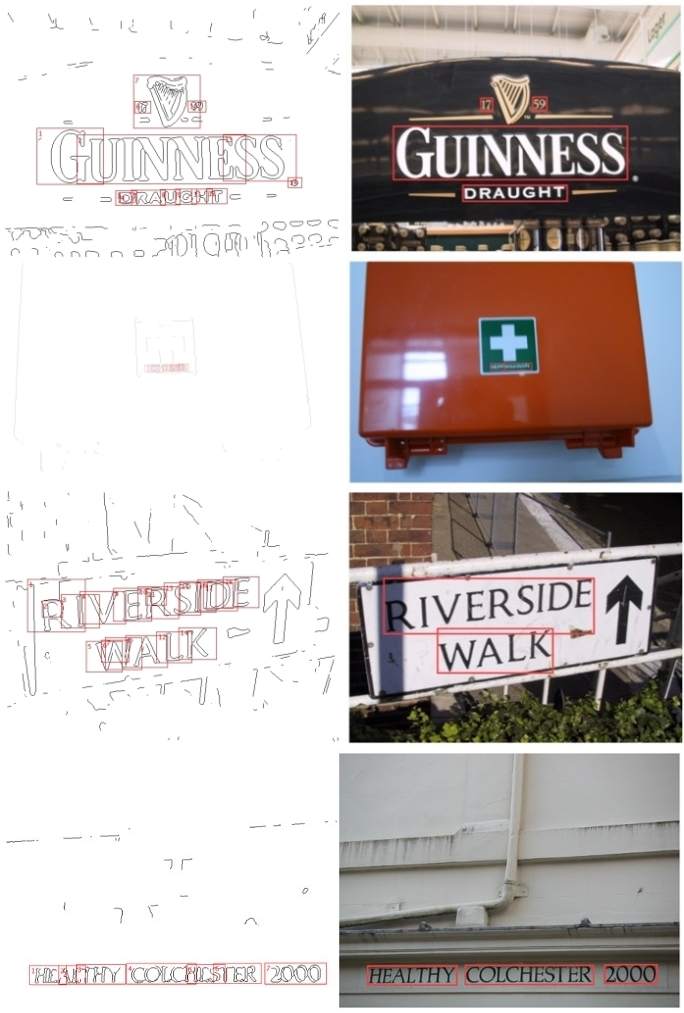
\includegraphics[width=\textwidth]{c3_ic13_results.jpg}
        \caption{ICDAR2013 上的测试结果示例}
        \label{fig.c3_ic13_results}
        \end{figure}

        \begin{figure}[!h]
        \centering
        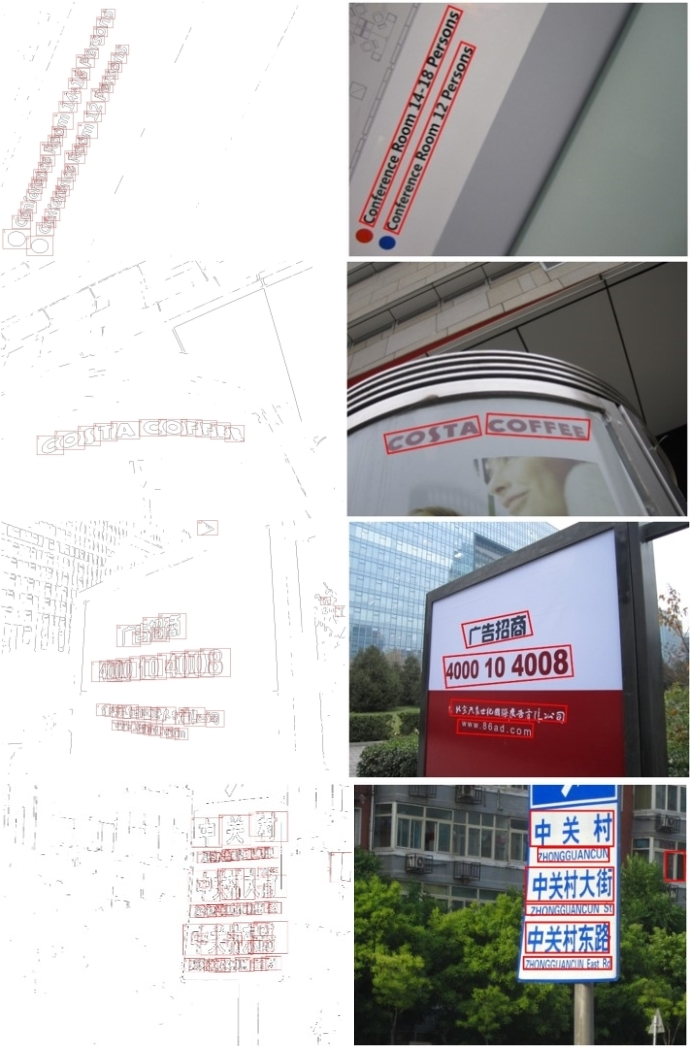
\includegraphics[width=\textwidth]{c3_msra_results.jpg}
        \caption{MSRA-TD500 上的测试结果示例}
        \label{fig.c3_msra_results}
        \end{figure}

    \section{本章小结}
    \esection{Brief Summary}

    本章提出的是基于边缘骨架切割的文字检测方法。首先对于输入的场景文字图片,利用结构化边缘检测方法得到边缘响应图,然后基于一系列像素强度值阈值,对边缘响应图进行分割,得到相应的二值化边缘图。接着在每个二值边缘图上,通过细化操作得到其边缘骨架图,并通过8 领域内像素点分析所找到的边缘骨架结点。而文字边缘与背景间的粘连点,就存在于这些边缘骨架结点中。因此断开粘连点得到候选的文字边缘骨架,然后经过形态学滤除来过滤掉大部分明显不是文字的边缘骨架,剩余的不易区分的非文字边缘骨架,可通过基于 CNN 的分类器来进一步滤除。最后基于非极大值抑制和文本行聚集操作,得到文本行定位结果。

    在公开数据集ICDAR2011,ICDAR2013以及MSRA-TD500上,我们对本章提出的方法都进行了实验,并将实验结果与其它先进方法进行了比较。实验结果证明了该方法的有效性。此外通过分析本章提出的方法,以及针对其文字定位包围盒不够精准的局限,我们将会在下一章中提出基于二叉树搜索的文本行优化方法。



        %% multiple1902 <multiple1902@gmail.com>
% intro.tex
% Copyright 2011~2012, multiple1902 (Weisi Dai)
% https://code.google.com/p/xjtuthesis/
%
% It is strongly recommended that you read documentations located at
%   http://code.google.com/p/xjtuthesis/wiki/Landing?tm=6
% in advance of your compilation if you have not read them before.
%
% This work may be distributed and/or modified under the
% conditions of the LaTeX Project Public License, either version 1.3
% of this license or (at your option) any later version.
% The latest version of this license is in
%   http://www.latex-project.org/lppl.txt
% and version 1.3 or later is part of all distributions of LaTeX
% version 2005/12/01 or later.
%
% This work has the LPPL maintenance status `maintained'.
%
% The Current Maintainer of this work is Weisi Dai.
%

\chapter{基于二叉树搜索的文字检测方法}
\echapter{Text detection based on Binary Tree Search}

    \section{问题的提出}
    \esection{Questions Posed}

    \section{方法原理与步骤}
    \esection{Principle and Summary of The Method}



    \section{候选文字行的提取}
    \esection{Candidate text line's extraction}

        \subsection{统计边缘响应}
        \esubsection{Static Skeleton Response}

        首先提出统计边缘响应方法,用以增强文本与背景之间的响应强度差异。给定如图\ref{fig.c4_static_skeleton_response}(a) 所示的场景文字图像$g$,计算其统计边缘响应$s$ 的方式如算法\ref{alg:c4_static_skeleton_response} 所示:

        \begin{algorithm} \renewcommand{\algorithmicrequire}{\textbf{输入:}}	\renewcommand{\algorithmicensure}{\textbf{输出:}}
    	\caption{统计边缘响应}
    	\label{alg:c4_static_skeleton_response}
    	\begin{algorithmic}[1]
    		\REQUIRE 输入的场景文字图像$g$
    		\ENSURE 图$g$相对应的统计边缘响应$s$
            \STATE 在图$g$上利用基于边缘骨架切割的文字检测子得到粗略的定位结果:文字定位包围框集合$B$及其相应的置信度分数集合$C$
    		\REPEAT
            \STATE $rs:=\left\{ b \times c  |\,b \in B, c \in C\right\}$
            \STATE $s:=s\cup rs,B:=B / b,C:=C / c$
            \UNTIL{$B=\varnothing$}
    	\end{algorithmic}
        \end{algorithm}

        其中$rs$指代的是响应小块,它的底面积是1 个定位包围框$b$,而高是$b$ 对应的置信度分数$c$。将所有的这些响应小块$rs$ 堆叠在一起,就构成了如图\ref{fig.c4_static_skeleton_response}(b) 所示的统计边缘响应$s$。

        \begin{figure}[!h]
        \begin{minipage}[t]{0.37\linewidth}
        \centering
        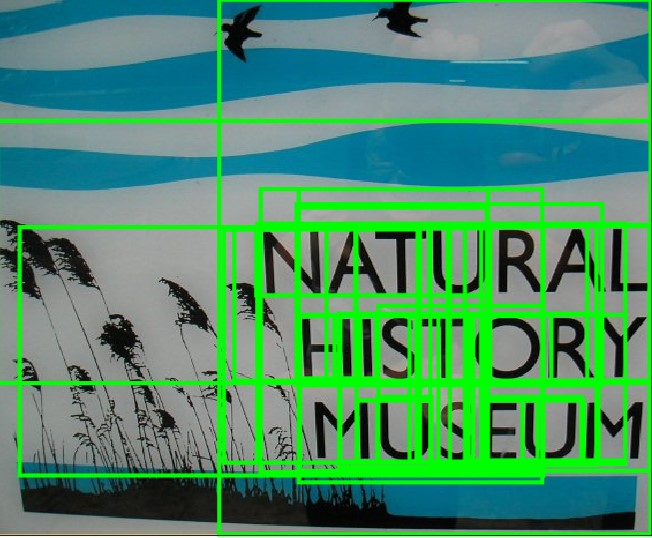
\includegraphics[width=\textwidth]{./figures/c4_img.jpg}
        \centerline{\small (a) 粗略定位结果}
        \end{minipage}
        \begin{minipage}[t]{0.35\linewidth}
        \centering
        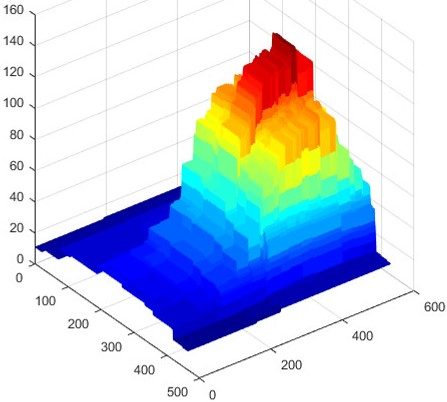
\includegraphics[width=\textwidth]{./figures/c4_static_skeleton_response.jpg}
        \centerline{\small (b) 统计边缘响应}
        \end{minipage}
        \begin{minipage}[t]{0.25\linewidth}
        \centering
        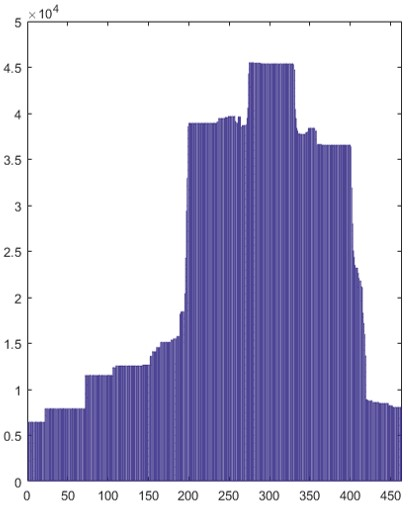
\includegraphics[width=\textwidth]{./figures/c4_horizontal_projection.jpg}
        \centerline{\small (c) 水平方向的映射}
        \end{minipage}
        \caption{在统计边缘响应中,文本区域与背景可以被区分开;而且通过后续的对统计边缘响应的水平映射操作,文本行也可以进一步区分开彼此}
        \label{fig.c4_static_skeleton_response}
        \end{figure}

        为了后续提取候选文本行的操作,首先要利用公式\ref{eq:c4_horizontal_projection} 来计算统计边缘响应$s$的横向投影$hp$,如图\ref{fig.c4_static_skeleton_response}(c) 所示。

        \begin{equation}
        hp= \left\{ \sum_{j=1}^w s_{ij} \, | \, i=1,2,...,h;j=1,2,...,w \right\},
        \label{eq:c4_horizontal_projection}
        \end{equation}

        其中,$h,w$分别是统计边缘响应$s$ 的高度和宽度。

        \subsection{候选文字行的生成}
        \esubsection{Text line's construction}

        在上1小节中得到了统计边缘响应$s$ 的横向投影$hp$, 它的数值如图\ref{fig.c4_candidate_line_construction}(a) 中的蓝色曲线所示,从中可看出候选文本行之间的响应有着明显的起伏变化。

        \begin{figure}[!h]
        \begin{minipage}[t]{0.32\linewidth}
        \centering
        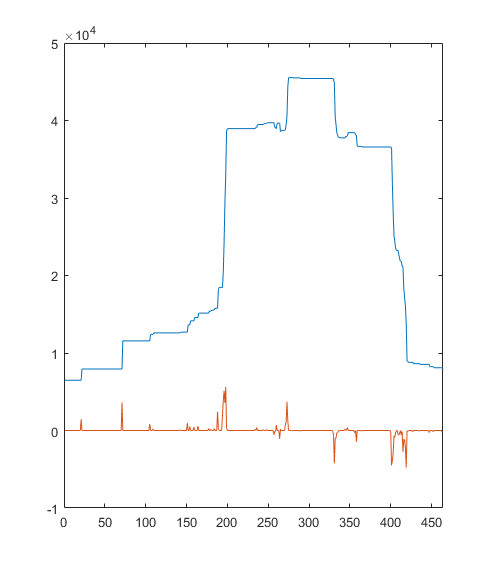
\includegraphics[width=\textwidth]{./figures/c4_gradient.jpg}
        \centerline{\small (a) 在水平映射图上的梯度}
        \end{minipage}
        \begin{minipage}[t]{0.32\linewidth}
        \centering
        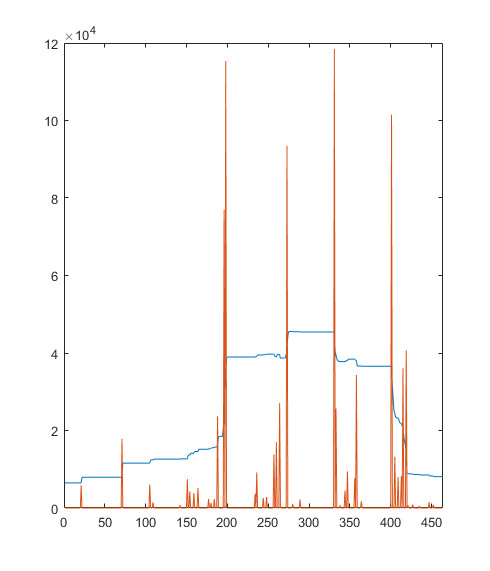
\includegraphics[width=\textwidth]{./figures/c4_unified.jpg}
        \centerline{\small (b) 梯度的取正和统一坐标}
        \end{minipage}
        \begin{minipage}[t]{0.32\linewidth}
        \centering
        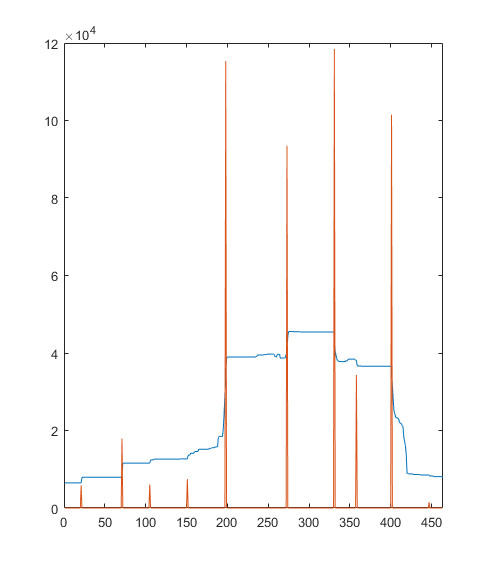
\includegraphics[width=\textwidth]{./figures/c4_nms.jpg}
        \centerline{\small (c) 梯度的非极大值抑制}
        \end{minipage}
        \caption{通过梯度计算和非极大值抑制操作来粗略定位文本行}
        \label{fig.c4_candidate_line_construction}
        \end{figure}

        为了确定候选文本行之间的分界线的具体位置,我们在统计边缘响应的横向投影$hp$上计算其梯度$g$,如图\ref{fig.c4_candidate_line_construction}(a) 中的脉冲状红线所示。梯度$g$表征着响应$hp$ 在某1 竖直位置上的变化程度:梯度$g$ 中的某1 脉冲状红线$l$ 的长度越大,就表明在红线$l$的附近越有可能存在着文字区域与背景区域之间的边界。而在梯度$g$中不存在脉冲红线的地方,意味着在这些区域的响应并没有发生突变,因此在$hp$ 上这些对应的位置上不存在文字区域与背景区域间的边界。

        为了便于观察和分析,首先对梯度值$g$取正,并将其提高至与$hp$统一的坐标内,如图\ref{fig.c4_candidate_line_construction}(b) 所示,这时得到的梯度值是$g$$'$。 最后在梯度值$g$$'$上执行非极大值抑制操作,由此消除掉绝大部分较小梯度值的无效脉冲状红线,并得到候选文本行集合$L$,而$L$ 由如图\ref{fig.c4_candidate_line_construction}(c) 中的$m$条红色候选文本行分割线组成。

    \section{二叉树型的文字行搜索空间的构建}
    \esection{Binary Tree-based search space's construction}

    将候选文本行集合$L$展现在场景文字原图上,如图\ref{fig.c4_binary_tree_construction}(b) 所示。$L$由$m$ 条红线$l_i, i=1,2,...,m$ 构成,这些红线是候选文本行分割线,并且在场景文字原图上分割出$m+1$个候选文本行条带,而这些文本行条带就是任两个相邻红线$l_i$和$l_{i+1}$ 之间的图像区域。那么现阶段的任务是,将所有候选文本行条带区域的排练组合作为1 个搜索空间,然后从中搜寻出最优的文本行条带组合,而这些条带区域能恰如其分地覆盖住文字所在的图像区域。

    \begin{figure}[!h]
    \centering
    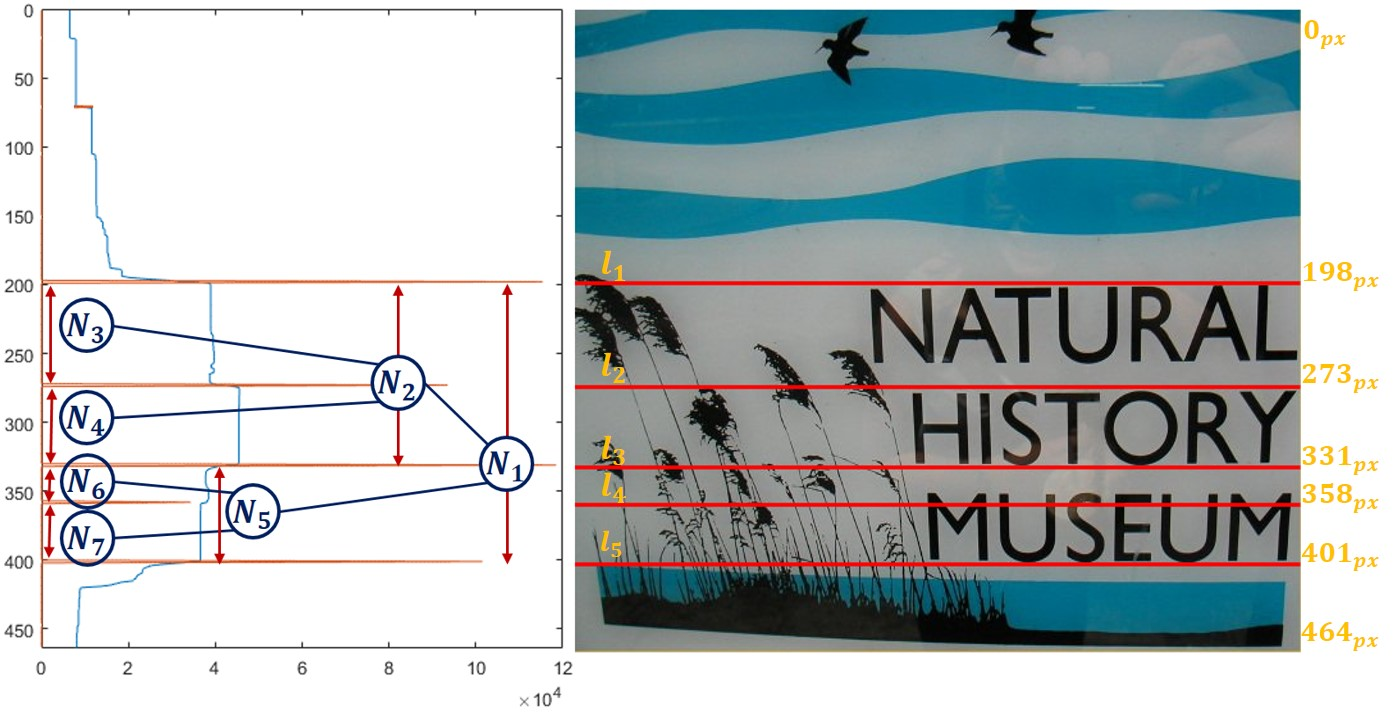
\includegraphics[width=\textwidth]{./figures/c4_binary_tree_construction.jpg}
    \begin{minipage}[t]{0.40\linewidth}
    \centerline{\small (a)二叉树型搜索空间}
    \end{minipage}
    \begin{minipage}[t]{0.51\linewidth}
    \centerline{\small(b)在场景图像中的候选文本行}
    \end{minipage}
    \caption{从候选文本行中建立起代表搜索空间的二叉树型数据结构}
    \label{fig.c4_binary_tree_construction}
    \end{figure}

    假设红色分割线$l_i$有2个属性:距离$ld_i$ 和置信度$lc_i$。其中属性$ld_i$ 指代的是从图像顶部到分割线$l_i$ 位置的距离,例如在图\ref{fig.c4_binary_tree_construction}(b) 中,$ld_3=331_{px}$就是指从图像顶部到线$l_3$的距离有331 个像素大小。而$lc_i$ 是分割线$l_i$的置信度,其数值是由$l_i$的梯度值归一化得到的,例如在图\ref{fig.c4_binary_tree_construction}(b) 中,$lc_3=0.987$ 表征的是$l_3$是文本行之间分割边界的可能性非常大。

    然后假设我们要构建的二叉树型搜索空间$N$是由一些结点$n$ 构成的。其中任一结点$n_i$有2 个对应的属性:结点代表的图像区域范围$nr_i$,以及结点的数值$nv_i$。以图\ref{fig.c4_binary_tree_construction}(a) 为例,节点$n_5$ 所代表的文本行区域范围是从线$l_3$ 到$l_5$之间的区域,而$n_5$的值是由$l_4$ 的置信度值$lc_4$ 赋予的。

    在明确候选文本行分割线$L$,以及二叉树型搜索空间$N$中各变量的含义后,由$L$构建$N$ 的过程如算法\ref{alg:c4_build_binary_tree} 所示:

    \begin{algorithm}[!h]
	\renewcommand{\algorithmicrequire}{\textbf{输入:}}
	\renewcommand{\algorithmicensure}{\textbf{输出:}}
	\caption{递归地建立二叉树型搜索空间}
	\label{alg:c4_build_binary_tree}
	\begin{algorithmic}[1]
		\REQUIRE 分割线 $L$ 的距离 $LD=\left\{ld_1,ld_2,...,ld_m\right\}$ 和置信度$LC=\left\{lc_1,lc_2,...,lc_m\right\}$
		\ENSURE 二叉树型搜索空间 $N$ 的结点范围 $NR=\left\{nr_1,nr_2,...,nr_{2m-3}\right\}$, 和结点的值 $NV=\left\{nv_1,nv_2,...,nv_{2m-3}\right\}$
      \STATE 初始化: \\
      \STATE \quad $i=0, \quad BuildBinaryTree(i,LD,LC)$
      \STATE function $BuildBinaryTree(i,LD,LC)$
        \\\STATE \quad $i=i+1$
        \\\STATE \quad $if \quad length(LD)==2 \quad then$
        \\\STATE \qquad $nr_{i}=[LD[1],LD[2]], nv_{i}=0$
        \\\STATE \qquad $return$
        \\\STATE \quad $end \ if$
        \\\STATE \quad $nr_{i}=[LD[1],LD[end]], nv_{i}=max(LC)$
        \\\STATE \quad $//$假设$LC$中的最大值是$lc_t$,其中$t$是$lc_t$ 的索引
        \\\STATE \quad $//$在索引$t$处将$L$分裂成左子集和右子集
        \\\STATE \quad $LD_{l}=\left\{LD[1],...,LD[t]\right\}, LC_{l}=\left\{LC[1],...,LC[t]\right\}$
        \\\STATE \quad $BuildBinaryTree(i,LD_{l},LC_{l})$
        \\\STATE \quad $LD_{r}=\left\{LD[t],...,LD[end]\right\}, LC_{r}=\left\{LC[t],...,LC[end]\right\}$
        \\\STATE \quad $BuildBinaryTree(i,LD_{r},LC_{r})$
      \STATE end function
	\end{algorithmic}
    \end{algorithm}

    那么,通过算法\ref{alg:c4_build_binary_tree} 从$L$中构建好的二叉树型搜索空间$N$就将存储在如图中的表格内。下一节,将介绍从搜索空间$N$ 中搜寻出最优文本行定位的搜索策略。

    \section{搜索最优的文字行定位}
    \esection{Searching the optimal text detection}

        \subsection{搜索路径}
        \esubsection{Searching the paths}

        给定二叉树型搜索空间$N$,假设$N$是由$m$ 个结点$n$ 构成,那么通过算法\ref{alg:c4_binary_tree_search},就可搜索出路径$P={p_1,p_2,...,p_{(m-1)/2}}$。 路径中的每个$p_i \in P$ 都是1个3元组:包含了父亲结点$np_i$,左子结点$nl_i$和右子结点$nr_i$。

        \begin{algorithm}[!h]
    	\renewcommand{\algorithmicrequire}{\textbf{输入:}}	
        \renewcommand{\algorithmicensure}{\textbf{输出:}}
    	\caption{从二叉树型搜索空间中找到最优路径}
    	\label{alg:c4_binary_tree_search}
    	\begin{algorithmic}[1]
    		\REQUIRE 二叉树型搜索空间 $N=\left\{n_1,n_2,...,n_m\right\}$, 其中每个结点$n_x \in N$有其相应的属性: 范围$nr_x$ 和值$nv_x$
    		\ENSURE 搜索到的路径 $P=\left\{p_1,p_2,...,p_{(m-1)/2}\right\}$, 其中每条路径$p_{i} \in P$ 包含结点三元组$p_{i}=\left\{np_{i},nl_{i},nr_{i}\right\}$

          \STATE 初始化: $idx=0$
          \FOR{$i=1$ to $(m-1)/2$}

          \FOR{$j=1$ to $m$}
          \IF{$nv_j$ == $leastPositive(NV)$}
          \STATE $np_i = n_j, nv_j = 0, idx = j$
          \ENDIF

          \IF{$nr_j[1]$ == $nr_{idx}[1]$ and $nv_j$ == $0$}
          \STATE $nl_i = n_j, nv_j = -1$
          \ENDIF

          \IF{$nr_j[2]$ == $nr_{idx}[2]$ and $nv_j$ == $0$}
          \STATE $nr_i = n_j, nv_j = -1$
          \ENDIF

          \ENDFOR

          \STATE $p_{i}$ = $\left\{ np_{i},nl_{i},nr_{i} \right\}$

          \ENDFOR
    	  \end{algorithmic}
        \end{algorithm}

        算法\ref{alg:c4_binary_tree_search} 的具体过程如下所述:根据二叉树的性质,如果二叉树$N$ 中存在$m$个结点,那么算法\ref{alg:c4_binary_tree_search} 就要迭代执行$(m-2)/2$ 次。在第$i$次迭代中:首先将具有最小正数值$nv_j \in NV$ 的结点$n_j \in N$,赋予路径三元组中的父亲结点$np_i$,并将$nv_j$ 设为0,从而使结点$n_j$转换为叶子结点;然后在二叉树$N$中寻找能赋予路径三元组中左子结点$nl_i$的1 个结点$n_x$,该结点必须满足下述条件:$n_x$的范围的左边界$nr_x$[1]须和$n_j$ 的范围的左边界$nr_j$[1] 相等,且其值$nv_x$ 须为0。那么找到满足要求的结点$n_x$,并将其赋予$nl_i$。 紧接着将该结点的值$nv_x$设为-1,这意味着结点$n_x$ 已被标注为``已处理'',也就是说结点$n_x$ 不会在算法的下一轮迭代中被考虑;类似地,搜索到$n_t$并将其赋予路径三元组中的右子结点$nr_i$,然后将$n_t$ 的值改为-1。

        以上过程是算法\ref{alg:c4_binary_tree_search} 的第i 次迭代。那么经过$(m-1)/2$次迭代后,包含$(m-1)/2$个三元组$p$的路径集合$P$就被构建了出来。

        \begin{figure}[!h]
        \centering
        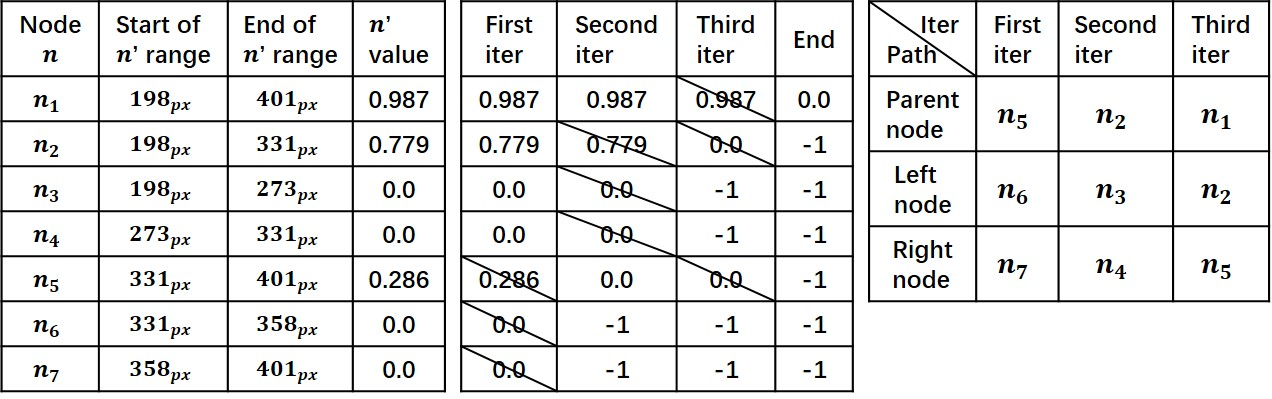
\includegraphics[width=\textwidth]{./figures/c4_bianry_tree_search.jpg}
        \begin{minipage}[t]{0.33\linewidth}
        \centerline{\small (a) 存储二叉树型搜索空间的表格}
        \end{minipage}
        \begin{minipage}[t]{0.33\linewidth}
        \centerline{\small(b)二叉树搜索算法的迭代过程}
        \end{minipage}
        \begin{minipage}[t]{0.26\linewidth}
        \centerline{\small(C)搜索到的路径结果}
        \end{minipage}
        \caption{1个从二叉树型搜索空间中找到最优路径的示例}
        \label{fig.c4_bianry_tree_search}
        \end{figure}

        为了更直观地理解算法\ref{alg:c4_binary_tree_search}:从二叉树型搜索空间中找到最优路径的算法,这里用图\ref{fig.c4_bianry_tree_search} 所示的例子加以阐述。首先图\ref{fig.c4_bianry_tree_search}(a) 中的表格存储的是代表候选文本行搜索空间的二叉树$N$,且在这个例子中,$N$含有7个结点;然后采用算法\ref{alg:c4_build_binary_tree} 在$N$上进行搜索,算法将会执行$(7-1)/2=3$ 次迭代,每次迭代的具体过程如图\ref{fig.c4_bianry_tree_search}(b) 所示;最后,算法的每次迭代,都会生成1 个对应的结点三元组。那么经历3 次迭代后,就会得到如图\ref{fig.c4_bianry_tree_search}(c) 所示的路径集合,即为算法\ref{alg:c4_binary_tree_search} 的搜索结果。

        \subsection{搜索策略}
        \esubsection{Searching strategies}
        \label{sec.c4_searching strategies}

        得到路径集合$P$后,在$P$上执行搜索策略,以得到最优的文本行定位。以图\ref{fig.c4_search_strategy}(a) 中的1 个被搜索到的路径三元组$p_i$为例,$p_i=\left\{np_i,nl_i,nr_i\right\}=\left\{n_5,n_6,n_7\right\}$。 那么对$p_1$的决策将在下列的3 项策略中选出并仅选出1种:

        (1)保留父亲结点$n_5$ 所代表的融合的文本行区域,而剪掉子结点$n_6$和$n_7$ 各自所代表的分离的文本行区域;

        (2)仅保留子结点$n_7$ 所代表的那部分单独的文本行区域,而剪掉父亲结点$n_5$ 所代表的融合的文本行区域以及子结点$n_6$ 所代表的单独的文本行区域;

        (2)仅保留子结点$n_6$ 所代表的那部分单独的文本行区域,而剪掉父亲结点$n_5$ 所代表的融合的文本行区域以及子结点$n_7$ 所代表的单独的文本行区域;

        对上述3种策略的选择过程是基于\ref{fig.c4_search_strategy}(b) 所示的2 阶段的判别步骤,而判别的依据是结点$n_6,n_7$ 以及$n_5$ 的识别成绩高低。这里采用的识别模型是Jaderberg等\cite{Jaderberg2016Reading} 的深度学习文字识别网络。我们按照结点的范围区域$nr$ 来截取出包含候选文本行的图块,将其输入文字识别网络,以得到该结点所代表文本行区域的识别成绩,并将其赋予结点的值$nv$。

        \begin{figure}[!h]
        \centering
        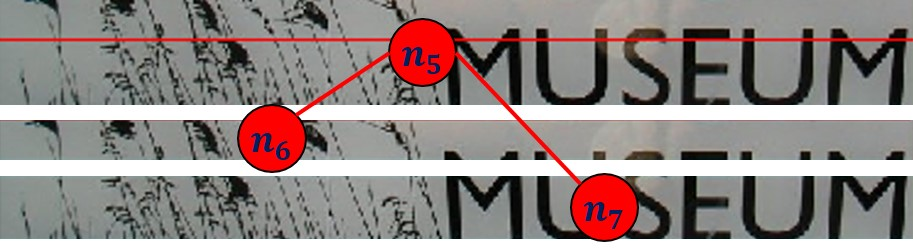
\includegraphics[width=\textwidth]{./figures/c4_search_strategy1.jpg}
        \centerline{\small (a) 1个被搜索到的路径三元组:其中每个结点代表1个候选文本行区域 }
        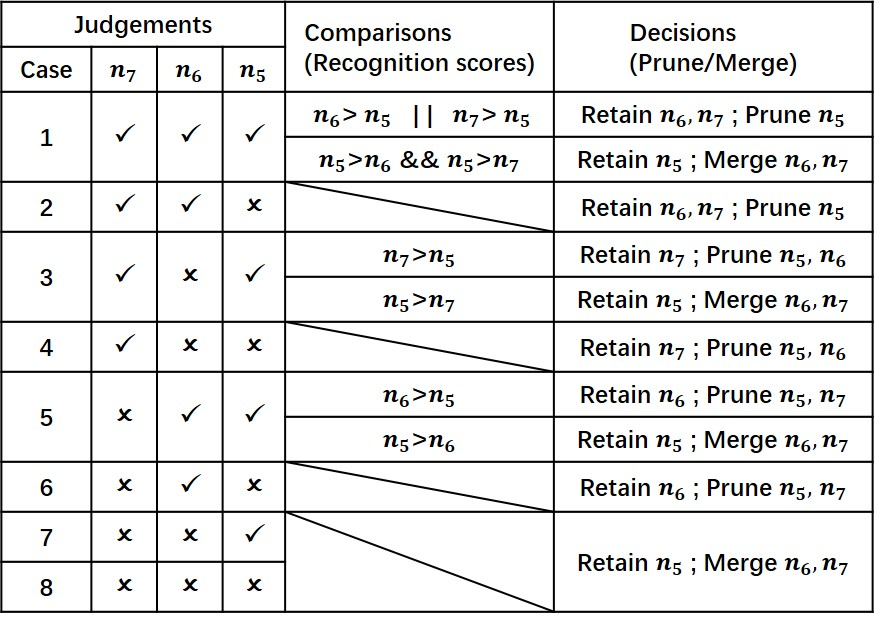
\includegraphics[width=\textwidth]{./figures/c4_search_strategy2.jpg}
        \centerline{\small (b) 对路径三元组的剪枝或融合策略}
        \caption{ 1个搜索策略的示例}
        \label{fig.c4_search_strategy}
        \end{figure}

        具体的2阶段判决过程如图\ref{fig.c4_search_strategy}(b) 所示:首先在第1阶段的判断过程中,结点$n_i$ 所代表的文字行区域要根据该结点的识别成绩值$nv$ 来进行而分类:如果$nv_i>0$,那么结点$n_i$ 所代表的区域被判定为文本行区域,并用对号标记;而如果$nv_i<0$,那么结点$n_i$所代表的区域被判定为非文本区域,并用错号标记。通过上述对3 个结点的二分类判断后,就会在$8=2^3$种情况中只选定1种情况条目进行后续的处理。然后在第2阶段的比较过程中,拿选定情况条目中的结点值$nv$进行对比,以此得到最终的决策结果。用图\ref{fig.c4_search_strategy}(b) 举例来说:假如$n_7$和$n_5$都被判定为文本,而$n_6$被判定为非文本,那么根据第1阶段的判定过程,选定情况条目3;然后在情况条目3中,经过第2 阶段比较过程,发现结点值$nv_5>nv_7$,那么得到最终的决策结果是:保留父亲结点$n_5$代表的融合的文本行区域,而剪掉子结点$n_6$和$n_7$ 各自所代表的分离的文本行区域。

        同理,下1条路径三元组$p_{i+1}=\left\{np_{i+1},nl_{i+1},nr_{i+1}\right\}$ 依然会在2阶段判决过程中得到自己相应的决策结果。那么重复该搜索策略,直到路径集合$P$ 中的所有路径三元组都经过处理而获得决策结果。最终,就获得了从二叉树型搜索空间中搜索得到的最优文本行定位结果。

    \section{实验和结果分析}
    \esection{Experimental Results}

        \subsection{实验数据集与评价标准}
        \esubsection{Data-set and Evaluation Protocol}

        为了验证本章提出的文字检测方法的效果和性能,我们将这个方法在ICDAR 2003(IC03),ICDAR 2011(IC11)以及ICDAR 2013(IC13)测试数据集上都运行并得到了结果。其中IC03,IC11和IC13各包含251,255及233张标注了文本的自然场景图像。这些测试数据集因其字体、颜色、尺度和光照的不同和变化而极具挑战性。

        最后将本方法与其它先进的文字检测和识别方法在谷歌街景数据集(Google Street View Text dataset,简称为SVT)进行了对比实验。SVT 文字测试集包含249张包含文字的街景图像。这些图像大多是模糊、光照不均的,并且数据集中的文字并未完全标注过,因此该文字检测数据集也充满了挑战。

        用以评价文字检测效果的标准依然是Wolf 等\cite{Wolf2006Object}提出的Object/area graphs 方法。其中对文字检测查全和查准率的计算公式如下所示:

        $recall = \frac {\sum_{i=1}^{|G|}Match_G(G_i,D,t_r,t_p)} {|G|}  ,   precision =\frac {\sum_{j=1}^{|D|}Match_G(D_j,G,t_r,t_p)} {|D|}$

        而文字检测的$f$值是查全recall和查准precision的均值。

        此外本章提出的方法还与其它方法在各场景文字图片数据集上进行了识别成绩的对比实验。用以验证识别效果的评判标准来自Wang\cite{Wang2012End}的方法。识别结果包含所有的拉丁文字,但是忽略那些不足3个字符长度的单词。只有当检测到的1个候选文字的包围框与文字定位结果真值(ground truth)的重叠率(Interaction over Union,简称为IoU)超过50\% 时,该候选文字的识别成绩才被认为是有效的。

        \subsection{实验结果与分析}
        \esubsection{Experimental Results and Analysis}

        如表格\ref{tab.c4_icdar13}所示,在自然场景文字图片数据集ICDAR 2013上,一些最先进的文字检测方法例如Cho\cite{Cho2016Canny} 的方法取得了81.1\%的检测F值,而我们的方法的检测F 值能达到82.3\%。其中,本章提出的方法取得了75.5\% 的查准率以及高达89.2\% 的查全率。本方法的查全率远高于其它先进的文字检测方法的查全率,原因就在于文本行的二叉树型搜索空间的建立,以及最优文本行搜索策略的执行。

        \begin{table}[!h]
        \centering
        \caption{在ICDAR 2013上的文字检测效果(\%)}
        \begin{tabular}{p{0.25\textwidth}|p{0.25\textwidth} p{0.25\textwidth} p{0.13\textwidth}}
        \hline
        方法 & 查全R & 查准P & F值 \\
        \hline
        \textbf{Proposed} & \textbf{89.2} & \textbf{75.5} & \textbf{82.3}\\
        He\cite{He2017scene} & 76.2 & 86.7 & 81.1 \\
        Cho\cite{Cho2016Canny} & 78.4 & 86.2 & 82.1 \\
        Tian\cite{Tian2016Text} & 75.8 & 85.1 & 80.2 \\
        Zhu\cite{Zhu2016Text} & 75 & 85 & 79 \\
        Gupta\cite{Gupta2016Synthetic} & 66.30 & 94.80 & 78.00 \\
        Pham\cite{Pham2016Robust} & 65.11 & 83.98 & 75.89 \\
        Neumann\cite{Neumann2012Real} & 64.84 & 87.51 & 74.49 \\
        \hline
        \end{tabular}
        \label{tab.c4_icdar13}
        \end{table}

        值得注意的是本章提出的方法是一种快速的文字检测算法,与Tian\cite{Tian2016Text} 的基于CNN的文字检测子相比,本方法消耗的是极小的计算量和时间。在ICDAR 2013的数据集中,平均的图像尺寸大约是1200乘以900个像素大小。而本章提出的方法平均处理一张图像大概只用0.76 秒左右,这其中包括了基于边缘骨架的文字检测子,统计边缘响应以及基于二叉树型搜索空间搜索的文本行优化等步骤的全过程。此外,与我们在上一章提出的方法即He\cite{He2017scene}的文字检测方法相比,本章新提出的基于二叉树搜索的文本行矫正方法,又使F 值提升了近2\%,由此证明该方法的确增强了文字检测的查全效果及查准效果。

        \begin{table}[!h]
        \centering
        \caption{在ICDAR 2011测试集上对于字符提取数目和检出率的测评}
        \begin{tabular}{p{0.33\textwidth}|p{0.33\textwidth} p{0.25\textwidth}}
        \hline
        方法 & 候选字符数目 & 检出率 \\
        \hline
        All ERs & 6,051,331 & 0.966 \\
        Matas\cite{Matas2004Robust} & 39,762 & 0.539 \\
        Sung\cite{Sung2015Scene} & 93,357 & 0.877  \\
        Cho\cite{Cho2016Canny} & 8,121 & 0.874 \\
        He\cite{He2017scene} & 8,231 & 0.879 \\
        \hline
        \textbf{Proposed} & \textbf{7,137} & \textbf{0.892} \\
        \hline
        \end{tabular}
        \label{tab.c4_icdar11}
        \end{table}

        如表\ref{tab.c4_icdar11}所示,在ICDAR 2011 文字测试数据集上,本章提出的基于二叉树搜索的文字检测方法与上一章提出的He\cite{He2017scene}的方法,以及其它最先进的的文字检测方法如Cho\cite{Cho2016Canny}、Sung\cite{Sung2015Scene} 等的方法都进行了字符提取数目和检出率的量化对比。从实验结果上来看,本章提出的方法可以在获得最高文字检出率的同时,保证提取的字符数目最少。该实验说明表明,相对于其它先进文字检测方法而言,本章方法都达到更优的文字查全和查准效果的折衷。

        \begin{figure}[!h]
        \centering
        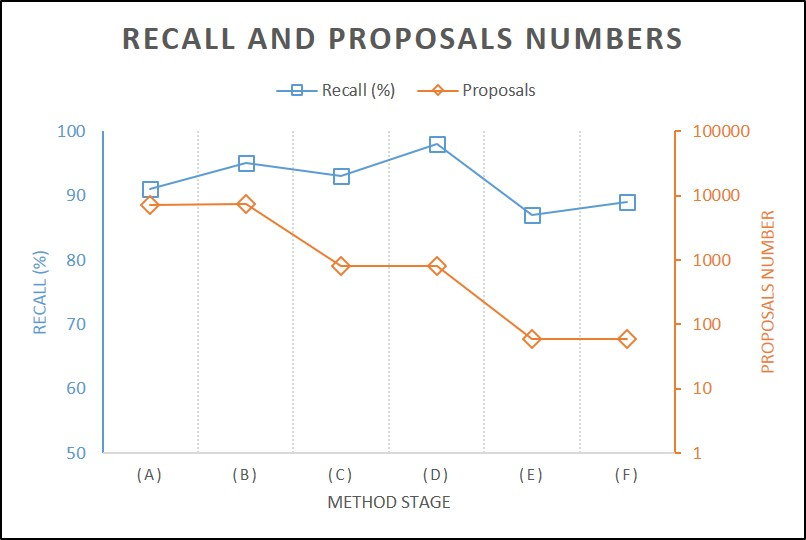
\includegraphics[width=\textwidth]{./figures/c4_recall_proposals.jpg}
        \caption{在ICDAR 2011 数据集上,本方法在各阶段中的文字检测查全与候选字符提取数目间的关系折线图: (a)候选文字边缘骨架提取, (b) 文字边缘骨架切割, (c)文字边缘骨架过滤, (d) 候选文本行定位, (e)非极大值抑制, (f) 基于二叉树搜索的文本行优化。}
        \label{fig.c4_recall_proposals}
        \end{figure}

        图\ref{fig.c4_recall_proposals}展示的是在本章提出方法的各阶段中,字符检出率与候选字符提取数目的关系折线图。与上一章提出的He\cite{He2017scene} 的方法相比,本章的方法在基于边缘骨架切割的文字检测子的基础上,融入了基于二叉树型搜索空间搜索的文本行定位优化方法。其中,基于二叉树搜索的文本行矫正进一步减少了非文字候选字符的提取数目,同时却提升了候选字符的查全效果。因此本章方法相对上一章方法,字符检出率增高2\%,且提取的候选字符数目能降低10\%。

        \begin{table*}[!h]
        \centering
        \caption{本章提出方法与其它先进方法的端对端文字识别成绩}
        \begin{tabular}{l|l l l l l l l}
        \hline
        方法 & IC03-50 & IC03-FULL & IC03 & SVT-50 & SVT & IC11 & IC13  \\
        \hline
        Neumann\cite{Neumann2010A} & -- & -- & 41 & -- & -- & -- & -- \\
        Wang\cite{Wang2012End} & 68 & 51 & -- & 38 & -- & -- & -- \\
        Wang\cite{Wang2012End} & 72 & 67 & -- & 46 & -- & -- & -- \\
        Matas\cite{Matas2014Scene} & -- & -- & -- & -- & -- & -- & 45 \\
        Alsharif\cite{Alsharif2013End} & 77 & 70 & 63 & 48 & -- & -- & -- \\
        Jaderberg\cite{Jaderberg2014Deep} & 80 & 75 & -- & -- & 56 & -- & -- \\
        Jaderberg\cite{Jaderberg2016Reading} & 90 & 86 & 78 & 76 & 53 & 76 & 76 \\
        He\cite{He2017scene} & 91 & 85 & 78 & 77 & 53 & 75 & 77 \\
        \textbf{Proposed} & 92 & 86 & 79 & 77 & 55 & 78 & 79 \\
        \hline
        \end{tabular}
        \label{tab.c4_recognition}
        \end{table*}

        在第\ref{sec.c4_searching strategies}节基于二叉树搜索的文本行优化的搜索策略中,我们详细探讨过自然场景文字检测与识别之间的紧密关系。其中,依据文字识别的成绩,文字检测的结果才能更准确的定位到文本行的位置。而反过来,更准确的文字检测结果,也会进一步的增强文字识别的精度。

        因此,我们也将本章提出的方法与其他方法在各场景文字图片数据集上做了识别成绩的对比实验,如表\ref{tab.c4_recognition} 所示。在所有的数据集上,本章提出的方法的端对端识别成绩都高于其它所有方法。在SVT-50数据集上,由Jaderberg\cite{Jaderberg2016Reading}提出的端对端识别模型获得了P/R/F(查准/查全/F值)分别为0.85/0.68/0.76的识别分数,而本章方法在这个成绩基础上继续提升5\%从而达到0.86/0.67/0.77的识别成绩。同样在IC03的各种词典配置的数据集上(IC03-50,IC03-FULL 和 IC03),本章方法相对于其它先进方法对F值的提升均在2\%左右,最终达到P/R/F分别为0.96/0.87/0.92的识别分数。




    \section{本章小结}
    \esection{Brief Summary}



        %% multiple1902 <multiple1902@gmail.com>
% intro.tex
% Copyright 2011~2012, multiple1902 (Weisi Dai)
% https://code.google.com/p/xjtuthesis/
%
% It is strongly recommended that you read documentations located at
%   http://code.google.com/p/xjtuthesis/wiki/Landing?tm=6
% in advance of your compilation if you have not read them before.
%
% This work may be distributed and/or modified under the
% conditions of the LaTeX Project Public License, either version 1.3
% of this license or (at your option) any later version.
% The latest version of this license is in
%   http://www.latex-project.org/lppl.txt
% and version 1.3 or later is part of all distributions of LaTeX
% version 2005/12/01 or later.
%
% This work has the LPPL maintenance status `maintained'.
%
% The Current Maintainer of this work is Weisi Dai.
%

\chapter{基于法向量的缺陷检测算法}
\echapter{Normal Vector based Defect Detection Method}

    \section{方法概述}
    \esection{Outline}
    

    

    \section{计算法向量梯度图}
    \esection{Gradient Map of Normal Vector}
   

    \section{双阈值分割}
    \esection{Dual Threshold Segmentation}
   
   

    \section{深度验证}
    \esection{Verification of Depth}
   
    \section{实验结果}
    \esection{Experimental Results}
        \subsection{数据集与评价方法}
        \esubsection{Data-set and Evaluation Protocol}
        
        \subsection{实验结果与分析}
        \esubsection{Experimental Results and Analysis}
        


    \section{本章小结}
    \esection{Brief Summary}
   


        % multiple1902 <multiple1902@gmail.com>
% conclusion.tex
% Copyright 2011~2012, multiple1902 (Weisi Dai)
% https://code.google.com/p/xjtuthesis/
%
% It is strongly recommended that you read documentations located at
%   http://code.google.com/p/xjtuthesis/wiki/Landing?tm=6
% in advance of your compilation if you have not read them before.
%
% This work may be distributed and/or modified under the
% conditions of the LaTeX Project Public License, either version 1.3
% of this license or (at your option) any later version.
% The latest version of this license is in
%   http://www.latex-project.org/lppl.txt
% and version 1.3 or later is part of all distributions of LaTeX
% version 2005/12/01 or later.
%
% This work has the LPPL maintenance status `maintained'.
%
% The Current Maintainer of this work is Weisi Dai.
%
\chapter{结论与展望}
\echapter{Conclusions and Future Work}
    \section{结论}
    \esection{Conclusions}
    连铸坯在高速、自动化的连续生产过程中,由于受原材料、轨制设备、系统控制等诸多技术因素的影响,导致连铸坯表面出现划伤、压痕、裂纹、结疤、刮伤等不同类型的缺陷。这些缺陷将会严重影响连铸坯的质量,使得连铸坯的抗腐蚀性、抗疲劳性、耐磨性等性能大大降低。这就要求连铸坯生产企业要对连铸坯进行充分的缺陷检测,保障连铸坯的质量,以减少在生产过程中可能发生的各类严重事故。因此,连铸坯表面的缺陷检测就成为连铸坯生产过程中极其重要的环节。本文的主要工作有:

    1)对现有的连铸坯表面缺陷检测方法进行了整理和总结,现有的连铸坯表面缺陷检测方法主要分为传统无损方法、基于RGB图像的方法和基于深度图像的方法。传统无损方法其主要使用一些钢板的物理特性,通过钢板对电、热、磁等反应的变化来探测缺陷,这些方法往往存在一些局限性,并且方法的实时性不高。基于RGB图像的方法是目前连铸坯表面缺陷检测的研究热点,这些方法主要是使用CCD相机采集钢板灰度图像,然后使用一些图像处理的手段来检测缺陷位置,然而这些算法对于伪缺陷的误检率较高。基于深度图像的方法主要是使用钢板的深度图像来检测缺陷,利用深度信息能够有效地检测出缺陷并排除伪缺陷。

    2)提出了一种基于显著性的缺陷检测方法,很好地解决了目前基于机器视觉的低对比度带黑斑缺陷检测难点,通过该方法,检测出的缺陷更加完整,误检数量明显减少,由于结合了改进的显著性检测方法,去除了图像中黑斑伪缺陷对检测结果的干扰,同时,该方法检测速度快,完全符合缺陷检测中对时间性能的要求。当然,该方法仍有继续研究和改进的空间,如何更加完整的提取到缺陷区域、更加完全的去除黑斑,以及时间性能的进一步提高都将成为接下来的工作重点。

    3)提出了一种基于基准面拟合的钢板深度图像缺陷检测算法。基于基准面的缺陷检测方法尝试去寻找钢板的基准面,然后将与基准面深度差别较大的区域作为缺陷种子点提取出来,最后使用基于种子点的图割方法来提取出完整的缺陷区域。另外,为了验证本文提出的两个缺陷检测算法,根据真实的钢板深度图像,我们使用人工合成的手段生成了一个钢板深度图像数据集,实验的结果显示,我们的方法达到了很好的效果。

    4)提出了一种基于法向量的深度图像缺陷检测算法。基于法向量的方法利用了缺陷部分的法向量变化较为剧烈这一特征,使用法向量梯度图像来刻画法向量的变化程度,概念上类似于灰度图像的梯度图,接着使用双阈值分割来获得候选缺陷区域,最终使用深度验证来确定候选缺陷区域是否为真正的缺陷。
    \section{展望}
    \esection{Future Work}
    本文一共提出了三种连铸坯钢板表面缺陷检测算法,其中,基于显著性图的缺陷检测算法是基于RGB图像的方法,基于基准面拟合的方法和基于法向量的方法是基于深度图像的方法。总结一下目前方法的不足之处,未来的工作主要集中在一下几点:

    1)对于基于显著性的方法,如何减少伪缺陷的误检率是关键,我们设计了一个流程来去除图像中的黑斑,但是对于钢板图像来说,伪缺陷除了黑斑还有氧化铁皮、水膜等等,如何改进算法使之对所有类型的伪缺陷都不产生误检同时对真正缺陷的检出率保持较高水平是未来的主要工作;

    2)需要收集连铸坯表面深度图像制作深度图像数据库,由于目前收集下载不到真实的连铸坯表面深度图像数据集,我们采用人工合成的手段制作了一个深度图像数据库,虽然在制作过程中我们尽可能地去拟合真实的钢板表面情况,但是在真正的连铸坯表面深度数据集上验证我们的算法的有效性还是有必要的;

    3)对于基于基准面拟合的方法,拟合出的基准面的质量直接决定了算法的缺陷检测性能,所以有必要对基准面拟合算法进一步研究和优化;

    4)对于基于法向量的方法,根据余弦相似度我们提出了一种法向量梯度图像来度量像素点之间法向量的差异,然而目前算法的查全率并不优秀,更改并设计一种新的度量方法来评价像素点之间法向量的差异是未来的主要研究内容。

    \xjtuendcontent

    % 将你要引用的文献的 BibTeX 放入 bibliography.bib
    \xjtubib{bibliography}

    \xjtuappendix
        % multiple1902 <multiple1902@gmail.com>
% appendice.tex
% Copyright 2011~2012, multiple1902 (Weisi Dai)
% https://code.google.com/p/xjtuthesis/
%
% It is strongly recommended that you read documentations located at
%   http://code.google.com/p/xjtuthesis/wiki/Landing?tm=6
% in advance of your compilation if you have not read them before.
%
% This work may be distributed and/or modified under the
% conditions of the LaTeX Project Public License, either version 1.3
% of this license or (at your option) any later version.
% The latest version of this license is in
%   http://www.latex-project.org/lppl.txt
% and version 1.3 or later is part of all distributions of LaTeX
% version 2005/12/01 or later.
%
% This work has the LPPL maintenance status `maintained'.
%
% The Current Maintainer of this work is Weisi Dai.
%

\iffalse
\xjtuappendixchapter{附录}
\xjtuappendixechapter{Appendices}
% 超过一个 section 时用 Appendices, 否则用 Appendix

    \xjtuappendixsection{二级标题}

        \xjtuappendixsubsection{三级标题}

            \xjtuappendixsubsubsection{四级标题}

    \xjtuappendixchapter{还是附录}

        \xjtuappendixsection{测试}
\fi

    \xjtuendappendix

    \xjtuspchapter{致谢}{致\qquad 谢}{Acknowledgements}
        % multiple1902 <multiple1902@gmail.com>
% acknowledgements.tex
% Copyright 2011~2012, multiple1902 (Weisi Dai)
% https://code.google.com/p/xjtuthesis/
%
% It is strongly recommended that you read documentations located at
%   http://code.google.com/p/xjtuthesis/wiki/Landing?tm=6
% in advance of your compilation if you have not read them before.
%
% This work may be distributed and/or modified under the
% conditions of the LaTeX Project Public License, either version 1.3
% of this license or (at your option) any later version.
% The latest version of this license is in
%   http://www.latex-project.org/lppl.txt
% and version 1.3 or later is part of all distributions of LaTeX
% version 2005/12/01 or later.
%
% This work has the LPPL maintenance status `maintained'.
%
% The Current Maintainer of this work is Weisi Dai.
%

研究生生活转眼就要接近尾声了,回首在西安交通大学七年的时光,心中倍感充实。我感谢这三年来老师们对我知识的传授、同学们对我友爱的表达,家人对我的亲切关怀。在此向所有支持和帮助过我的人表示由衷的感谢。

我首先想感谢的是我的指导老师,宋永红老师和张元林老师。从我的论文选题、开题、撰写、到论文的定稿,这一路走来,每一步都离不开老师的谆谆教诲和悉心关怀。两位老师治学严谨、知识渊博、谦虚平和,与老师的每一次谈话都让我受益匪浅。老师教会我的不仅是做学问的态度,更重要的是为人处事的方式,我将带着这些在接下来的工作和生活中继续努力,让自己变得更加优秀。

感谢施乐组所有的兄弟姐妹:王晓兵师兄、张云师兄、郁冲师兄、龚晨师兄、梁朝寓师兄、冯媛媛师姐、李伟师兄、尚玉飞师兄、陈奇师兄、段露师姐、刘衍峰师兄、魏盛华、赵路、张值、戴觊婧、李晓玉、杜鹏、任泽宇、吴晨、杨柳、张晗、陈敬军、米泽双、王鑫、魏儒波。因为有你们,我才有三年丰富的研究生生活。

感谢我的家人为我的付出和对我无微不至的关怀,为我创造了如此优越的学习和生活环境。无论我身在何方,开心或是沮丧,成功或是失败,你们都在我背后默默支持着我、鼓励着我。你们是我奋斗的动力,我会努力让你们为我骄傲。

最后,衷心感谢在百忙之中抽出时间评阅本论文的专家们, 不足之处,请批评指正。


    \xjtuspchapter{攻读硕士期间取得的研究成果}{攻读硕士期间取得的研究成果}{Achievements}
        % multiple1902 <multiple1902@gmail.com>
% acknowledgements.tex
% Copyright 2011~2012, multiple1902 (Weisi Dai)
% https://code.google.com/p/xjtuthesis/
%
% It is strongly recommended that you read documentations located at
%   http://code.google.com/p/xjtuthesis/wiki/Landing?tm=6
% in advance of your compilation if you have not read them before.
%
% This work may be distributed and/or modified under the
% conditions of the LaTeX Project Public License, either version 1.3
% of this license or (at your option) any later version.
% The latest version of this license is in
%   http://www.latex-project.org/lppl.txt
% and version 1.3 or later is part of all distributions of LaTeX
% version 2005/12/01 or later.
%
% This work has the LPPL maintenance status `maintained'.
%
% The Current Maintainer of this work is Weisi Dai.
%
【论文与专利】

[1]宋永红,贺翔,张元林.一种基于二叉树的文本行精确定位方法[P].中国发明专利,申请号:2016108504496

[2]宋永红,贺翔,张元林.一种用以增强文字与背景差异的边缘响应统计变换方法[P].中国发明专利,申请号:2016108503972

[3]He Xiang, Song Yonghong, Zhang Yuanlin. Scene Text Detection based on Statistic Edge Response and MSER, 25th National Conference on Multimedia Technology(NCMT),2016.

[4]He Xiang, Song Yonghong, Zhang Yuanlin. Scene Text Detection based on Skeleton-cut Detector, 24th International Conference on Image Processing(ICIP),2017.

[5]He Xiang, Song Yonghong, Zhang Yuanlin. A coarse-to-fine scene text detection method based on Skeleton-cut detector and Binary-Tree-Search based rectification, Pattern Recognition Letters, 2018已投稿



【参与项目】

[1]海尔智能冰箱中的容器包装文字识别项目(2017.6 - 2017.12) 项目组长

本项目目标是在低分辨率冰箱摄像头拍摄的图片中,检测并识别出食品包装上的有用信息。首先利用基于深度网络的目标检测方法来定位文字,然后采用CRNN模型对定位到的文字进行识别,此外引入基于ReID的图像匹配算法来辅助提升识别效果。本人负责完成的工作有:制订工作计划、调研相关工作、仿真算法、制作数据集、实现算法、设计和搭建系统平台、做实验测试结果、调试系统以及在每个阶段撰写技术报告。



%\clearpage




    \xjtuacademicintegrity


\end{document}
